\documentclass[a4paper, 12pt]{article}

\title{
{\large Topological Data Analysis -- group project} \\
	\vspace{3mm}
	\hrule
	\vspace{3mm}
Sensors
	\vspace{3mm}
	\hrule
}

\author{
	Nejc Ki\v sek,
	\v Zan Klane\v cek
}

\usepackage[utf8x]{inputenc}
\usepackage{float}
\usepackage{graphicx}
\usepackage{subcaption}
\usepackage{geometry}
\usepackage{amsfonts}
\usepackage{amsmath}
\usepackage{amssymb}
\usepackage{hyperref}
\newcommand{\vect}[1]{\boldsymbol{#1}}


\begin{document}
\maketitle


\section{Introduction}
In this project we are trying to find optimal parameters for a sensor network which covers the whole surface of the earth. The network is determined by two parameters: 
\begin{itemize}
	\item $r$, which is the distance over which the sensors can communicate with each other -- each sensor can communicate with other, if they are at most $r$ away.
	\item $R$, which is the radius of the surrounding are in shape of a circle where the sensor can gather data.
\end{itemize}

\noindent Given the coordinates of each sensor, we had to determine the lowest possible parameters $r$ and $R$ so that:

\begin{itemize}
	\item {the sensor network is connected,}
	\item {the sensor network covers the whole sphere (surface of the Earth).}
\end{itemize}
Furthermore, once the parameters $r$ and $R$ are established, obsolete sensors should be removed. These are sensors whose removal would not change the connectivity and coverage of the sensor network. Lastly, a data generator that distributes $n$ points evenly on the surface of a sphere will be described. With this generator, parameters $r$ and $R$ of the sensor network will be as small as possible.
\section{Topological solution}

In this section theoretical background for our problem is described. Firstly, if we want to achieve sensor network connectivity (all sensors are connected), we should have a look at Vietoris-Rips complex. Such $r$ (as small as possible) should be determined, that Vietoris-Rips graph on a given distribution of sensors is connected (i.e. has one component). The properties of Vietoris-Rips are described with following relations:

\begin{itemize}
	\item {sensors: S $\big(S_i = (r_i, \phi_i, \theta_i)\big)$,}
	\item {sensor connections $\{S_i, S_j\} \subset S; d(S_i, S_j) \leq 2r$,}
	\item {$F \subset S$ is a simplex in $VR_r(S)$, if diam $F \leq 2r$,}
\end{itemize} 
where $r$ is yet unknown parameter of sensor network and $d(S_i, S_j)$ is Euclidean distance between two sensors. 
Secondly, if we want to achieve coverage of the entire sphere, Čech complex characteristics will come in handy:

\begin{itemize}
	\item {sensors: S $\big(S_i = (r_i, \phi_i, \theta_i)\big)$,}
	\item {$B_R(x)$ closed ball with radius $R$ around $x$,}
	\item {$C_R = \{\sigma \subset S,\cap_{x\in \sigma}B_R(x) \neq \emptyset \}$.
	}
\end{itemize}
In this case, such $R$ (as small as possible) should be determined, so that the Euler characteristic of the Čech complex is the same as that of a sphere. However, in practice, we rather determined first two Betti numbers which should be equal to 1 and 0, meaning there is only one component with no holes. 
\clearpage
\section{Distribution of sensors}
In Figure 1 the pre-given distribution of sensors is visualized. The major difference between distribution of points in sensors01 and sensors02 is around the poles.
\begin{figure}[H]
        \centering
        \makebox[\linewidth][c]{
        	\centering
            \begin{subfigure}[b]{0.55\textwidth}
                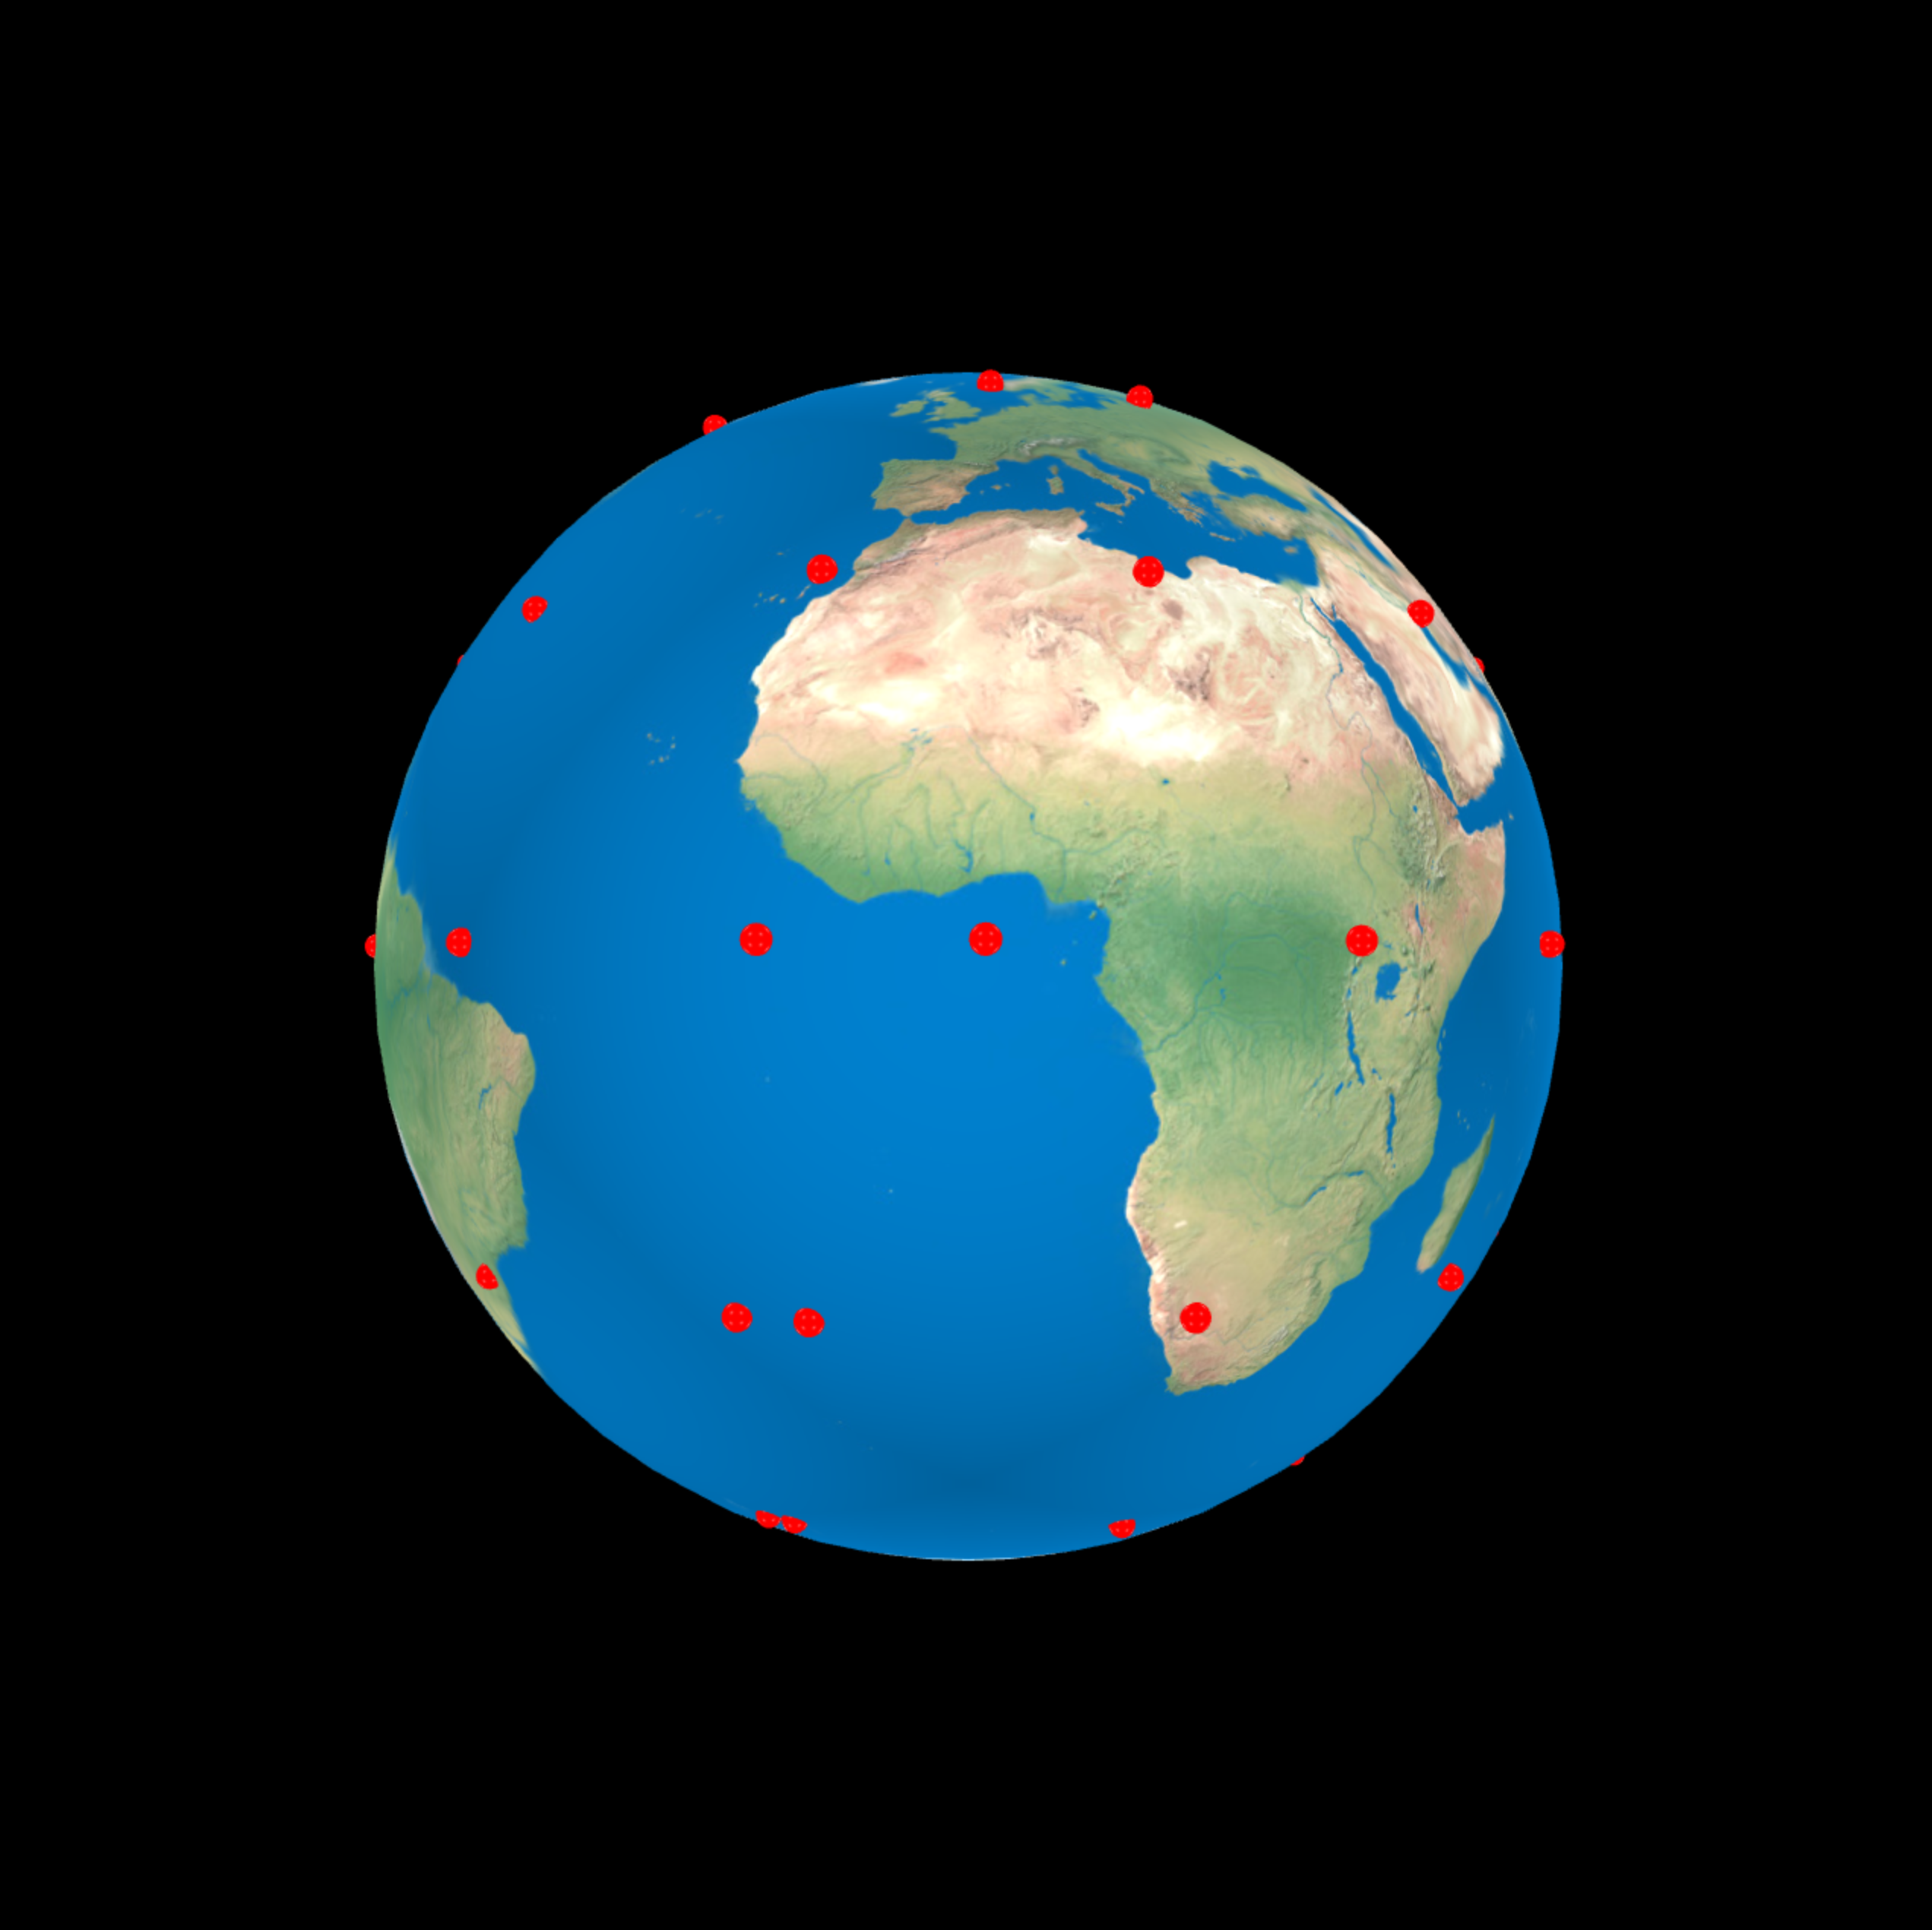
\includegraphics[width=\textwidth]{../images/sensors01}
                \caption{sensors01.txt}
            \end{subfigure}
            \begin{subfigure}[b]{0.55\textwidth}
                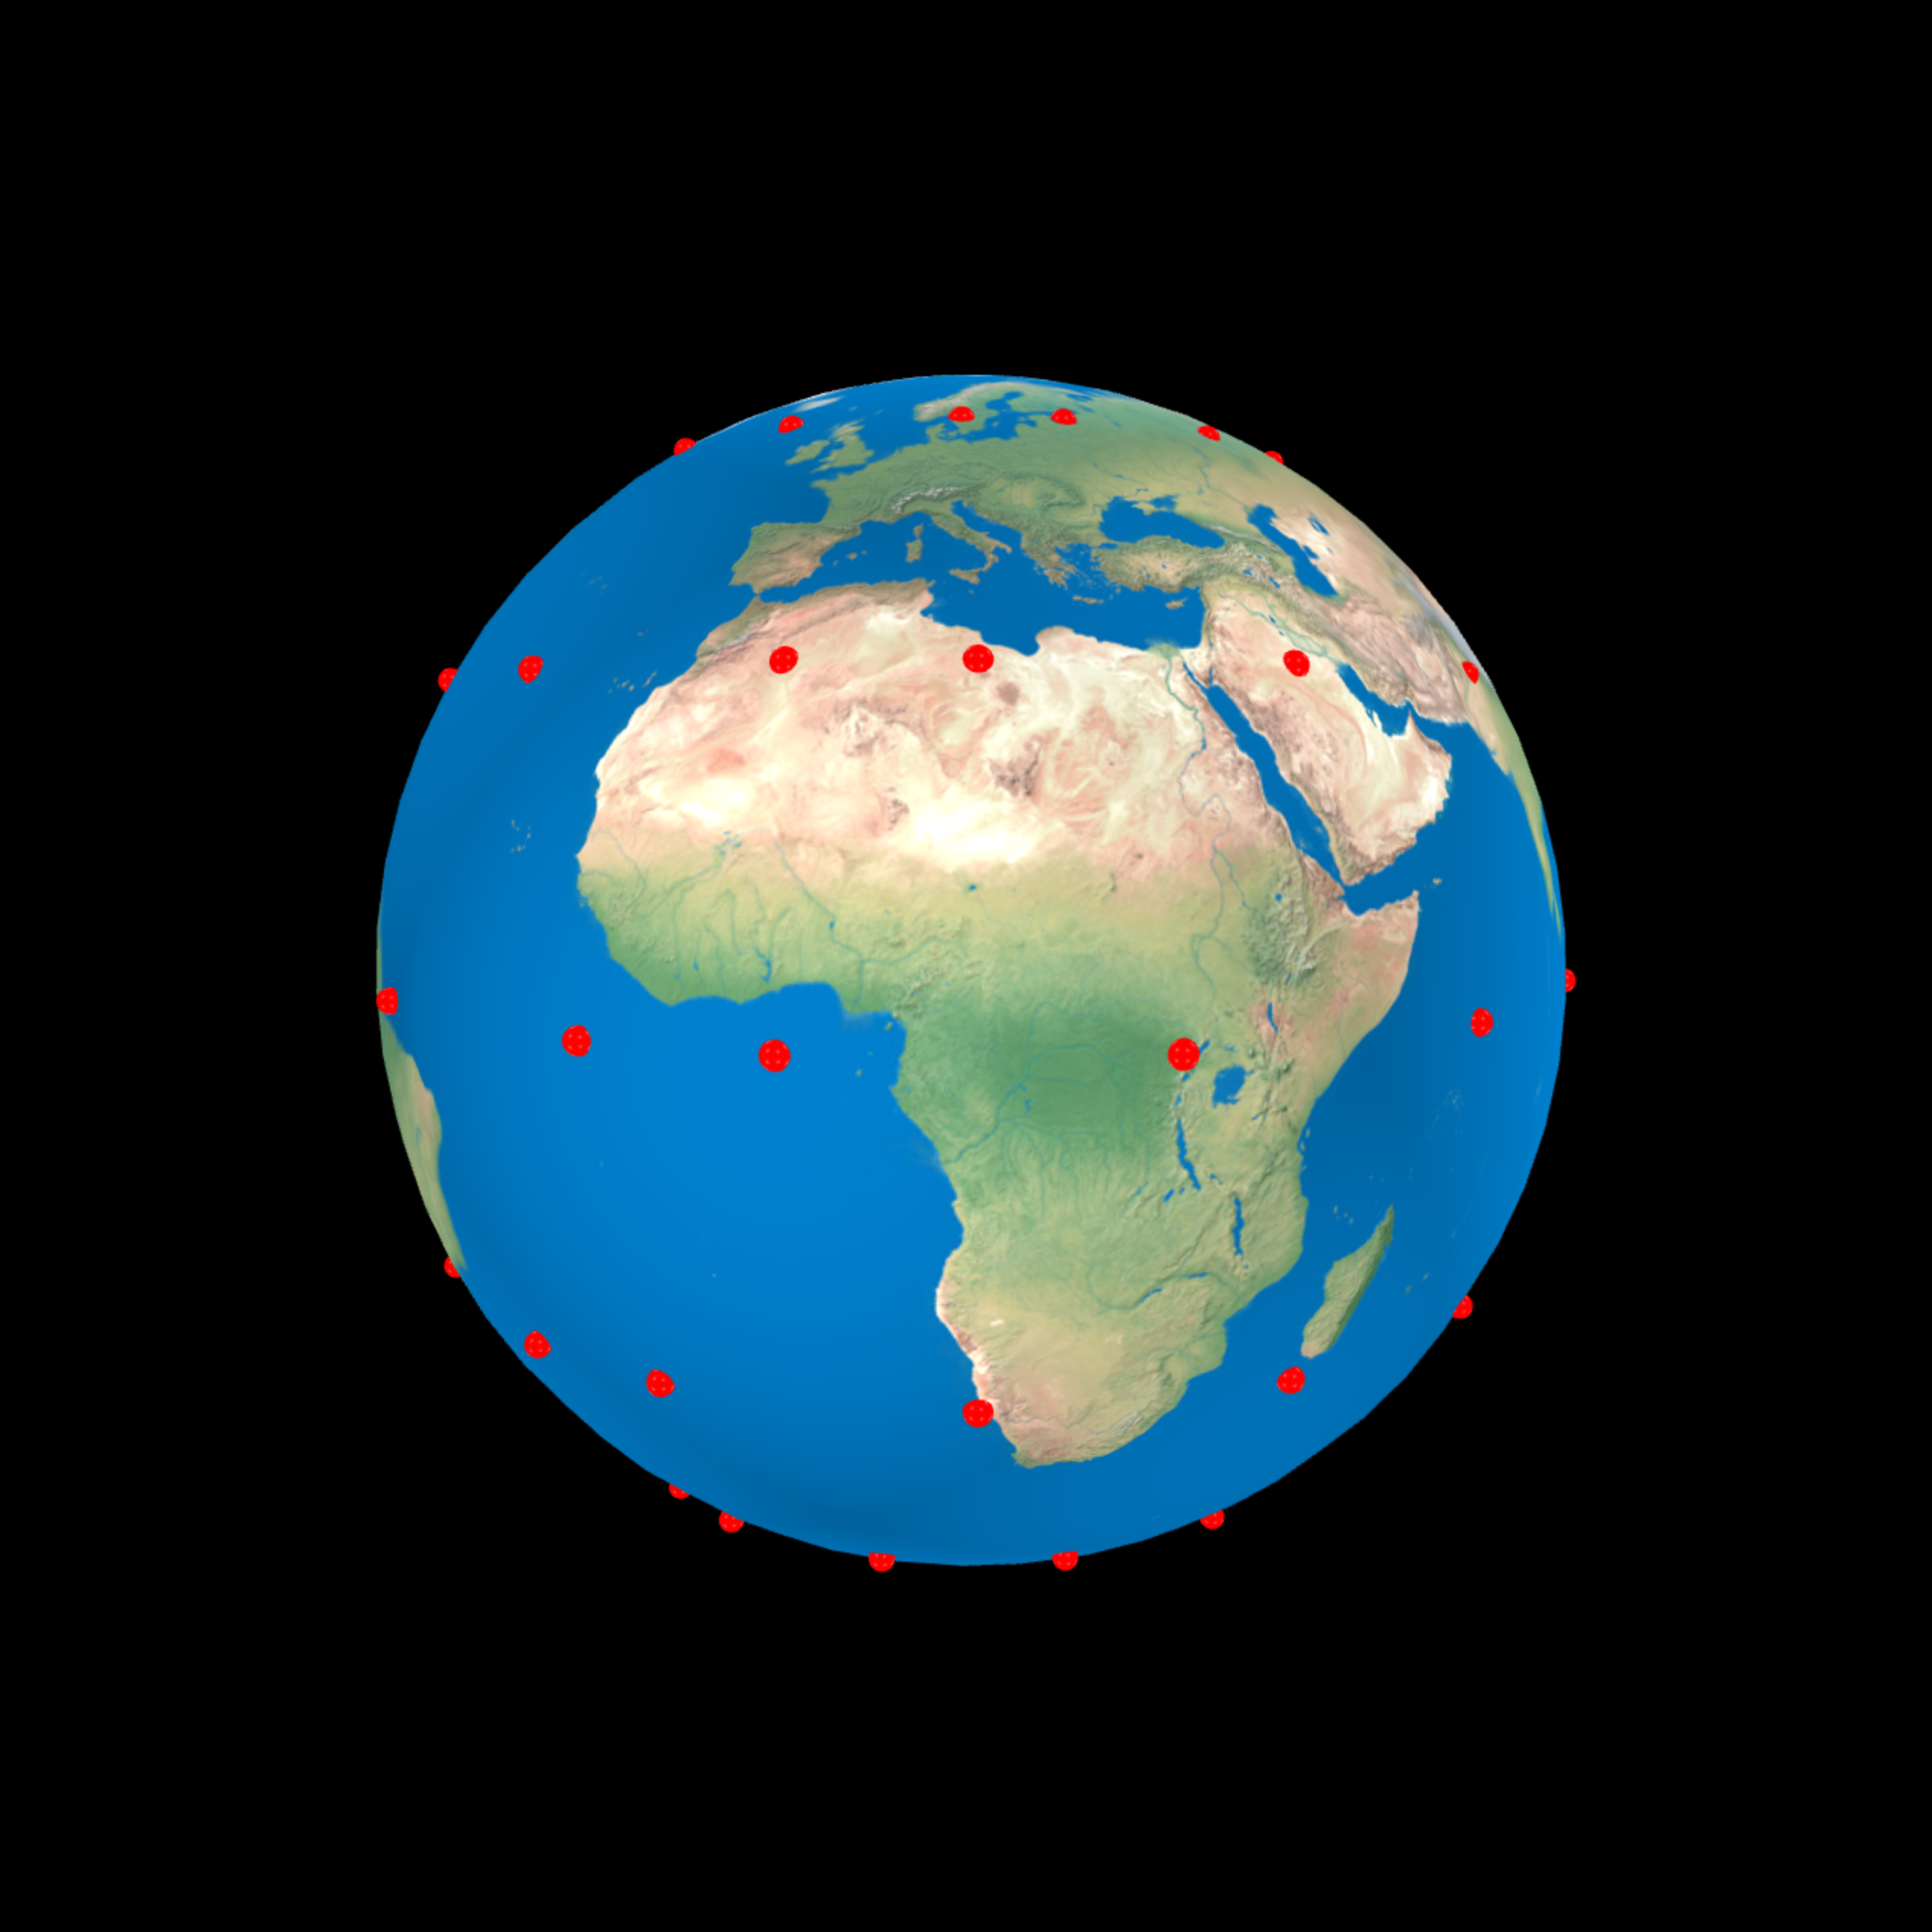
\includegraphics[width=\textwidth]{../images/sensors02}
                \caption{sensors02.txt}
            \end{subfigure}
        }
        \caption{Locations of the sensors}
\end{figure}

\section{Connectivity}
TODO: VR complex, increasing $r$ until we get 1 component. 

\begin{figure}[H]
        \centering
        \makebox[\linewidth][c]{
        	\centering
            \begin{subfigure}[b]{0.6\textwidth}
                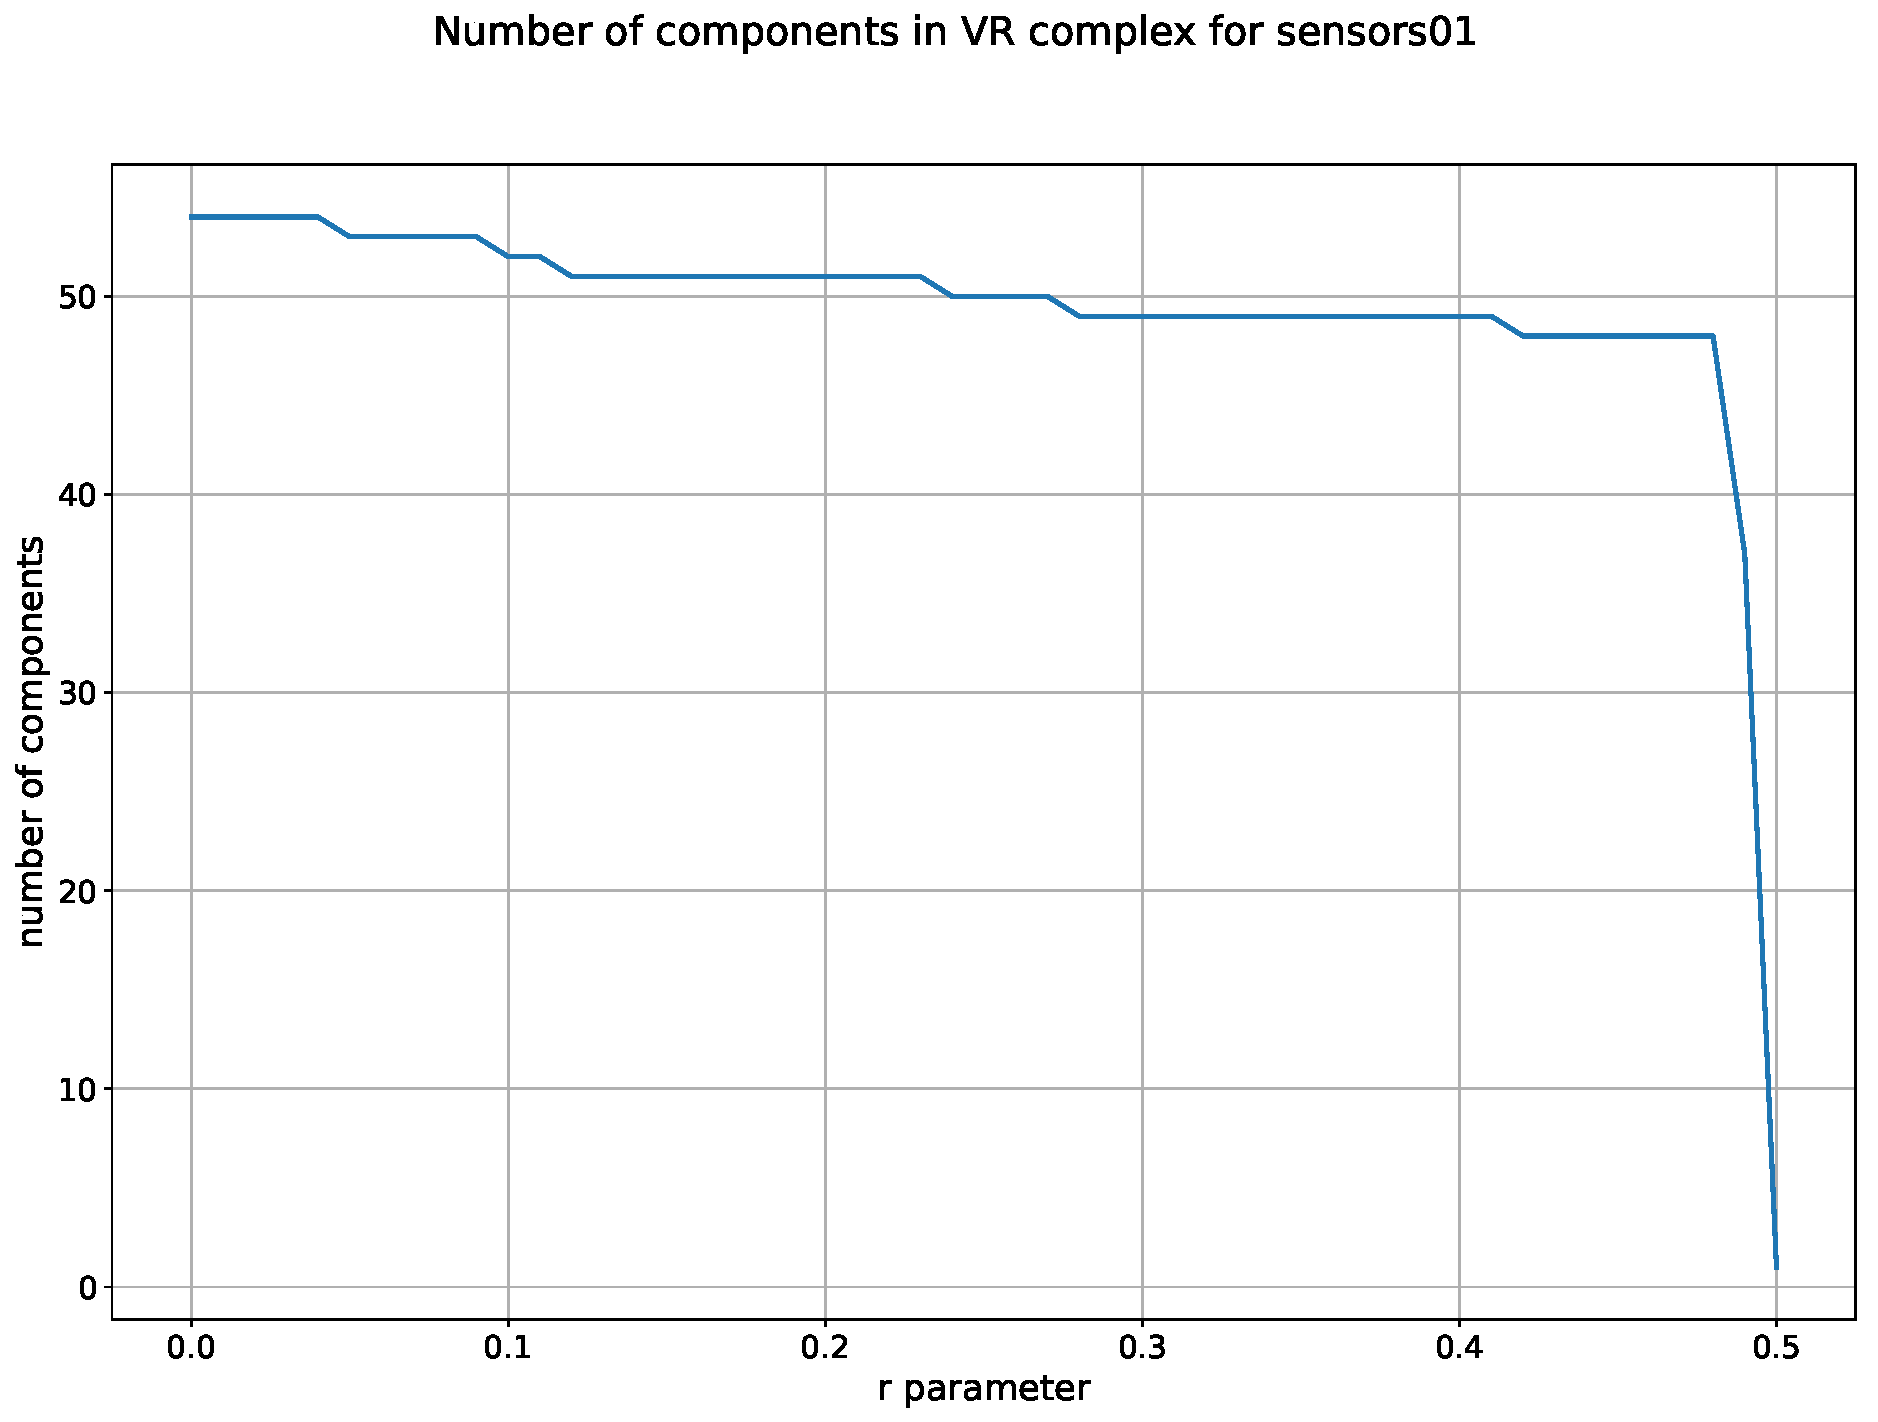
\includegraphics[width=\textwidth]{../images/plot_vr_sensors01}
            \end{subfigure}
            \begin{subfigure}[b]{0.6\textwidth}
                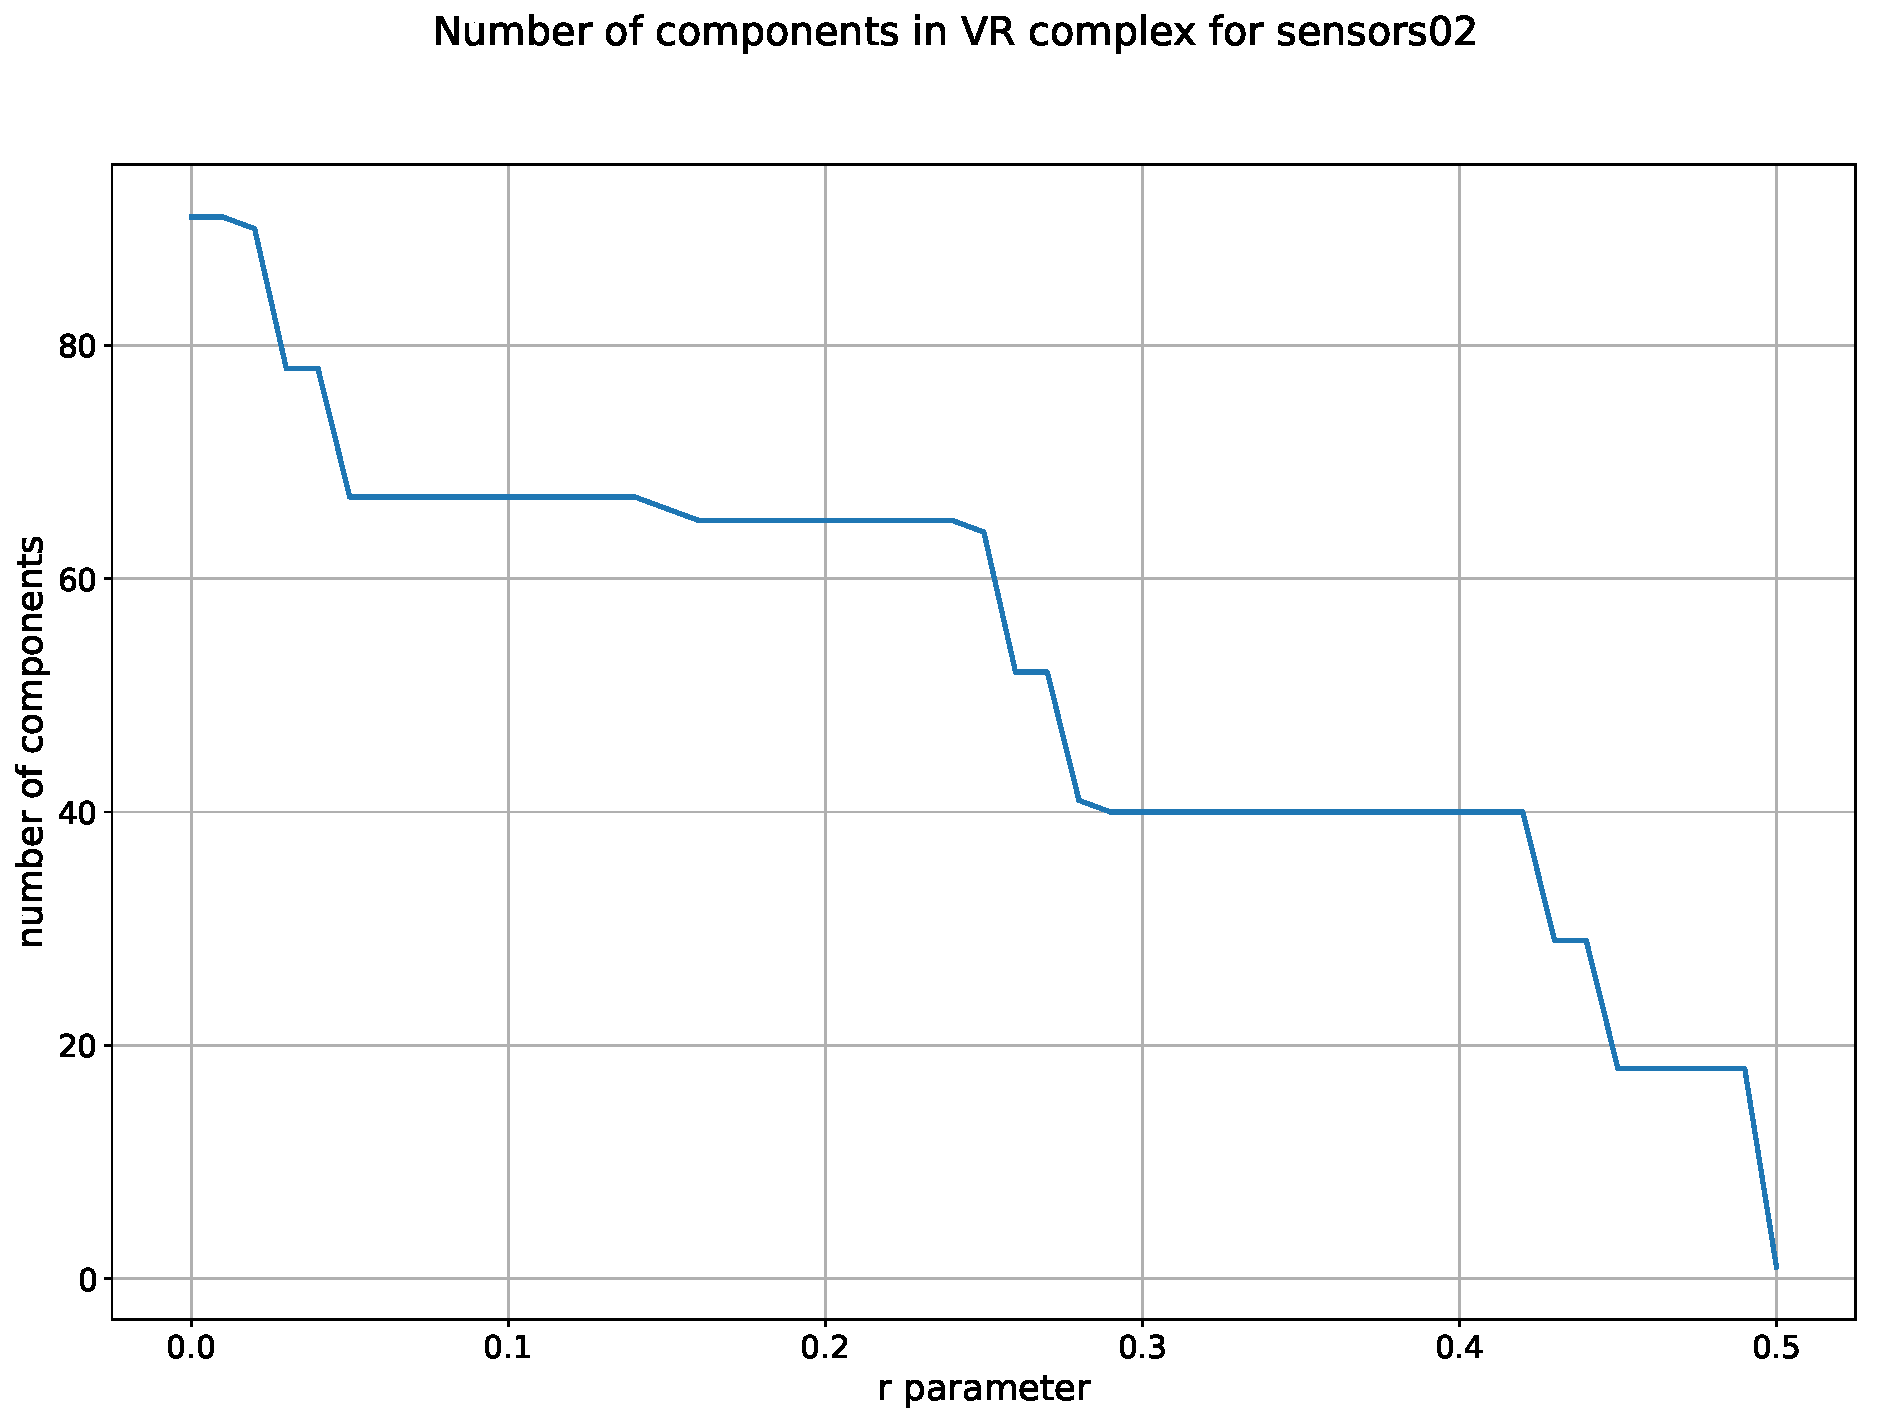
\includegraphics[width=\textwidth]{../images/plot_vr_sensors02}
            \end{subfigure}
        }
        \caption{Number of components as we increase the $r$ parameter}
\end{figure}

TODO: malo komentarja na graf

\begin{figure}[H]
        \centering
        \makebox[\linewidth][c]{
        	\centering
            \begin{subfigure}[b]{0.55\textwidth}
                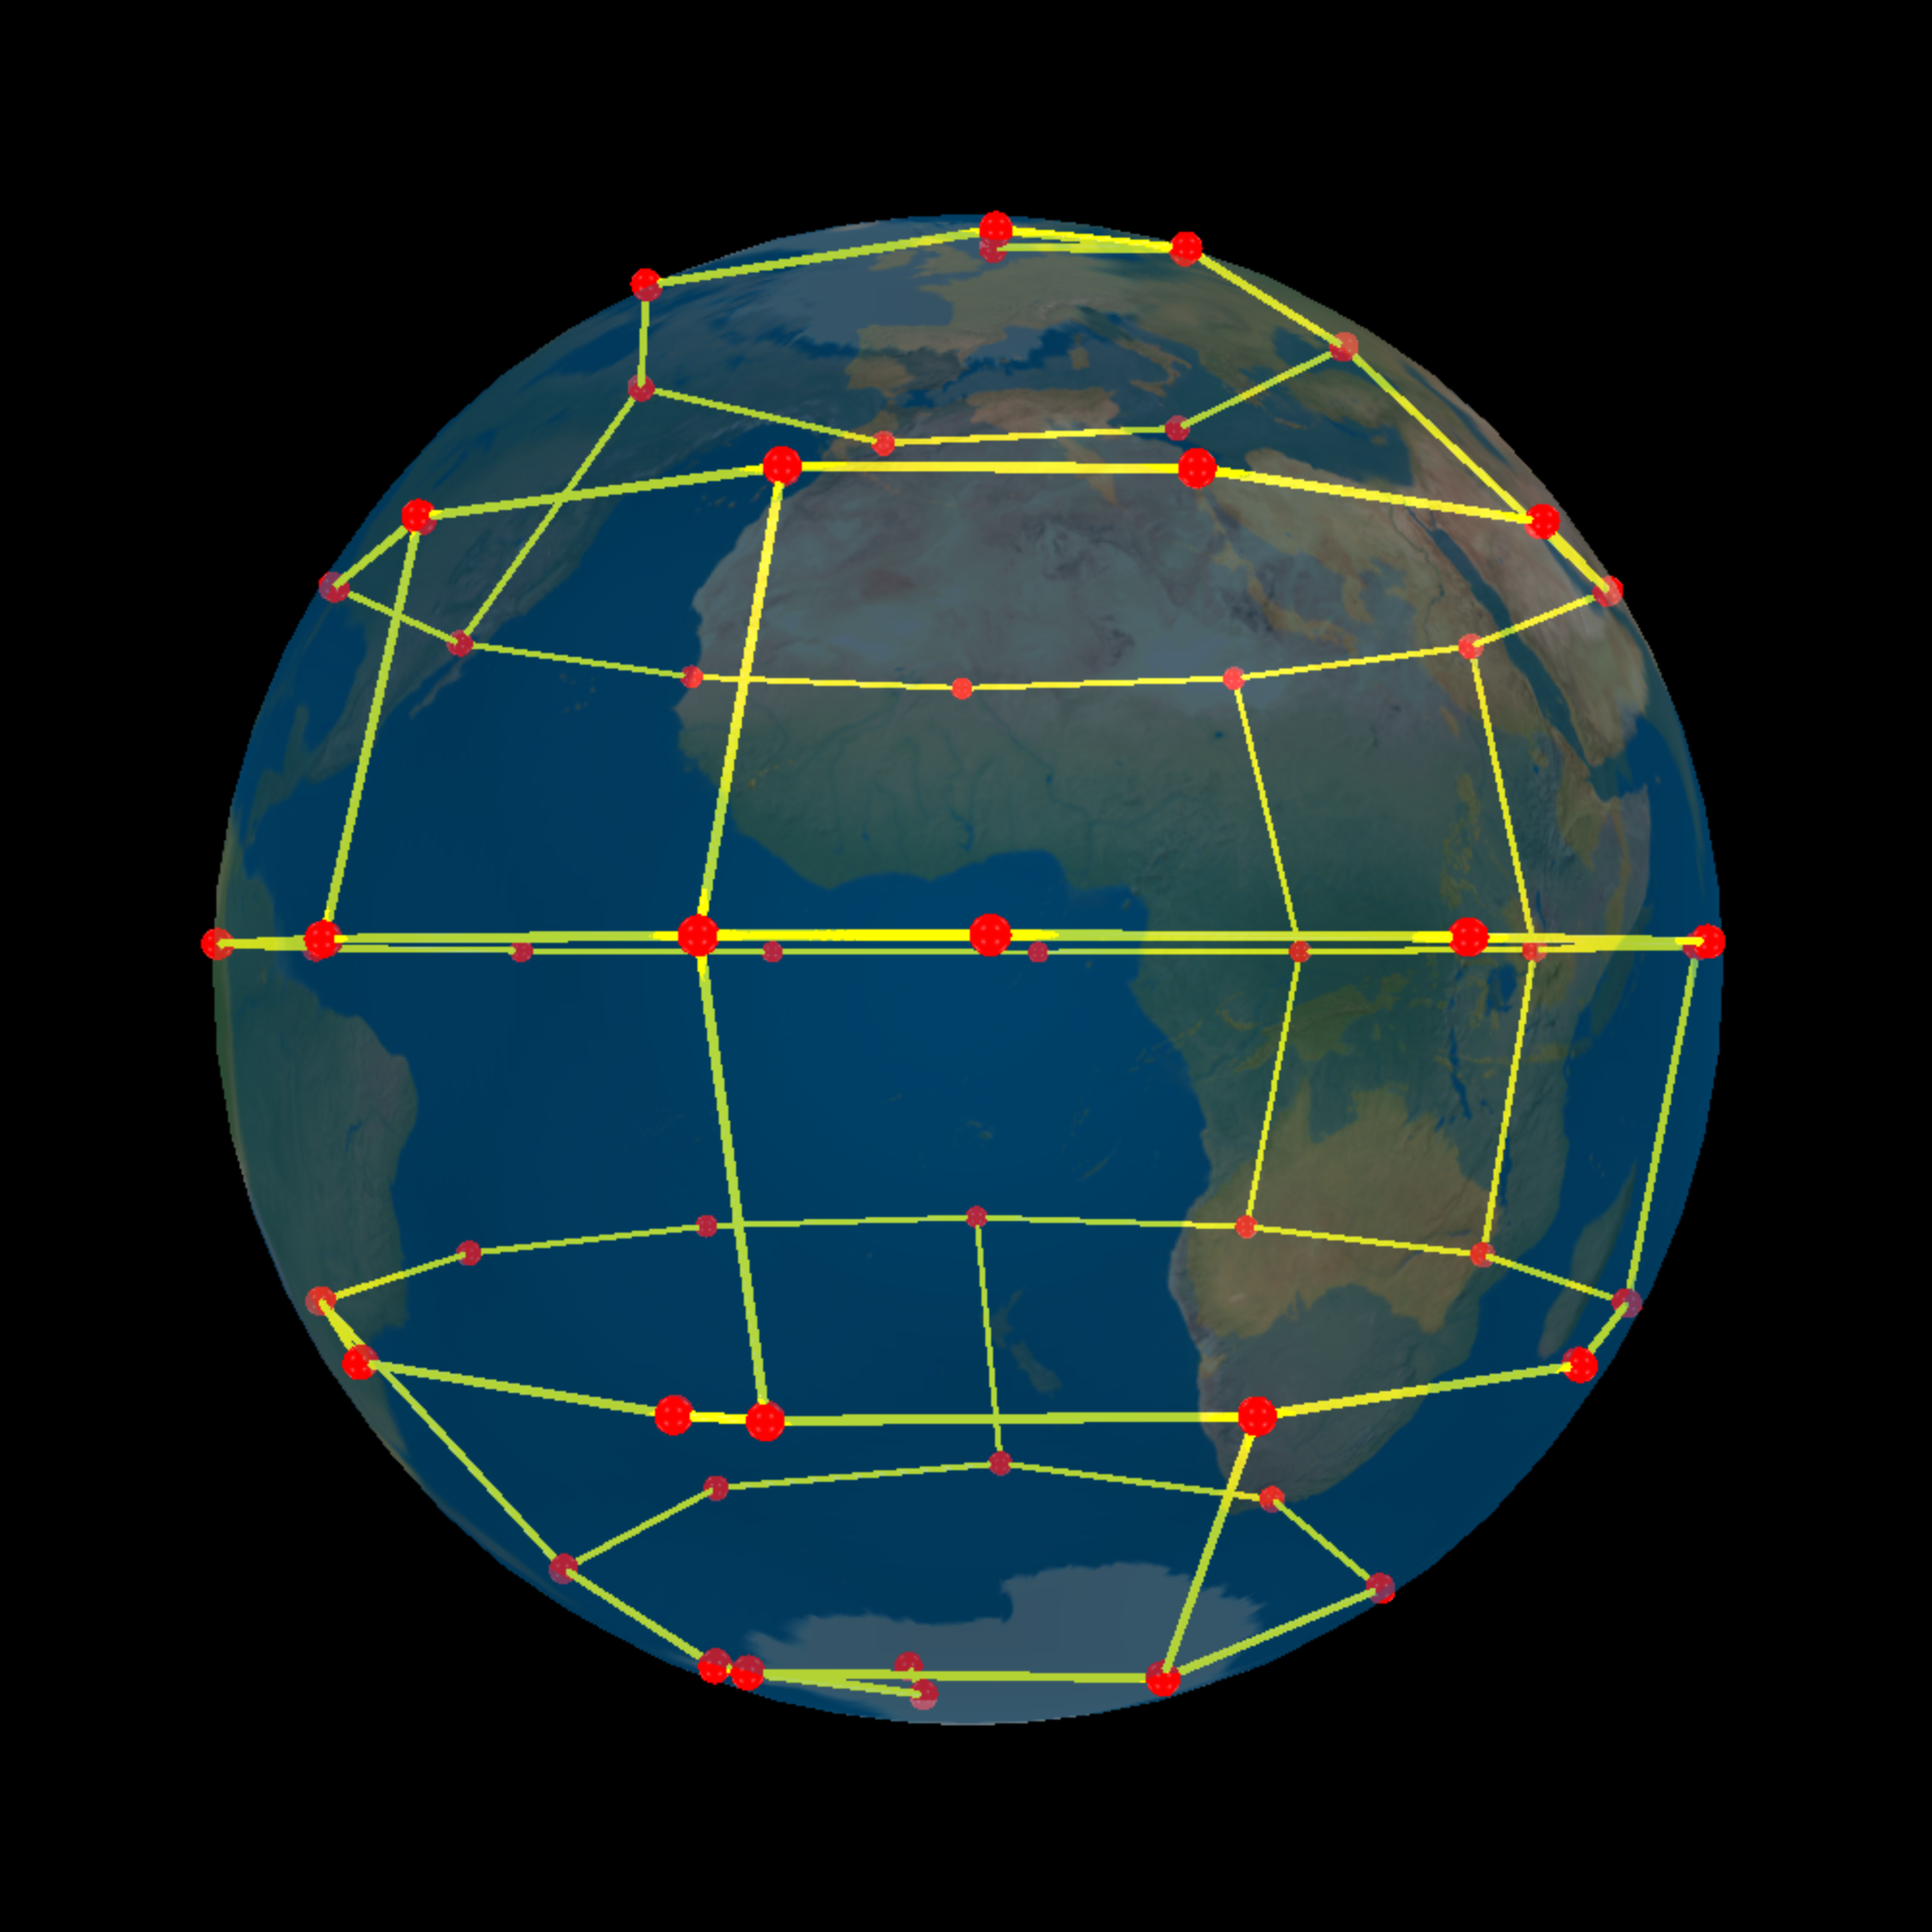
\includegraphics[width=\textwidth]{../images/connections01}
                \caption{sensors01.txt ($r=0.5$)}
            \end{subfigure}
            \begin{subfigure}[b]{0.55\textwidth}
                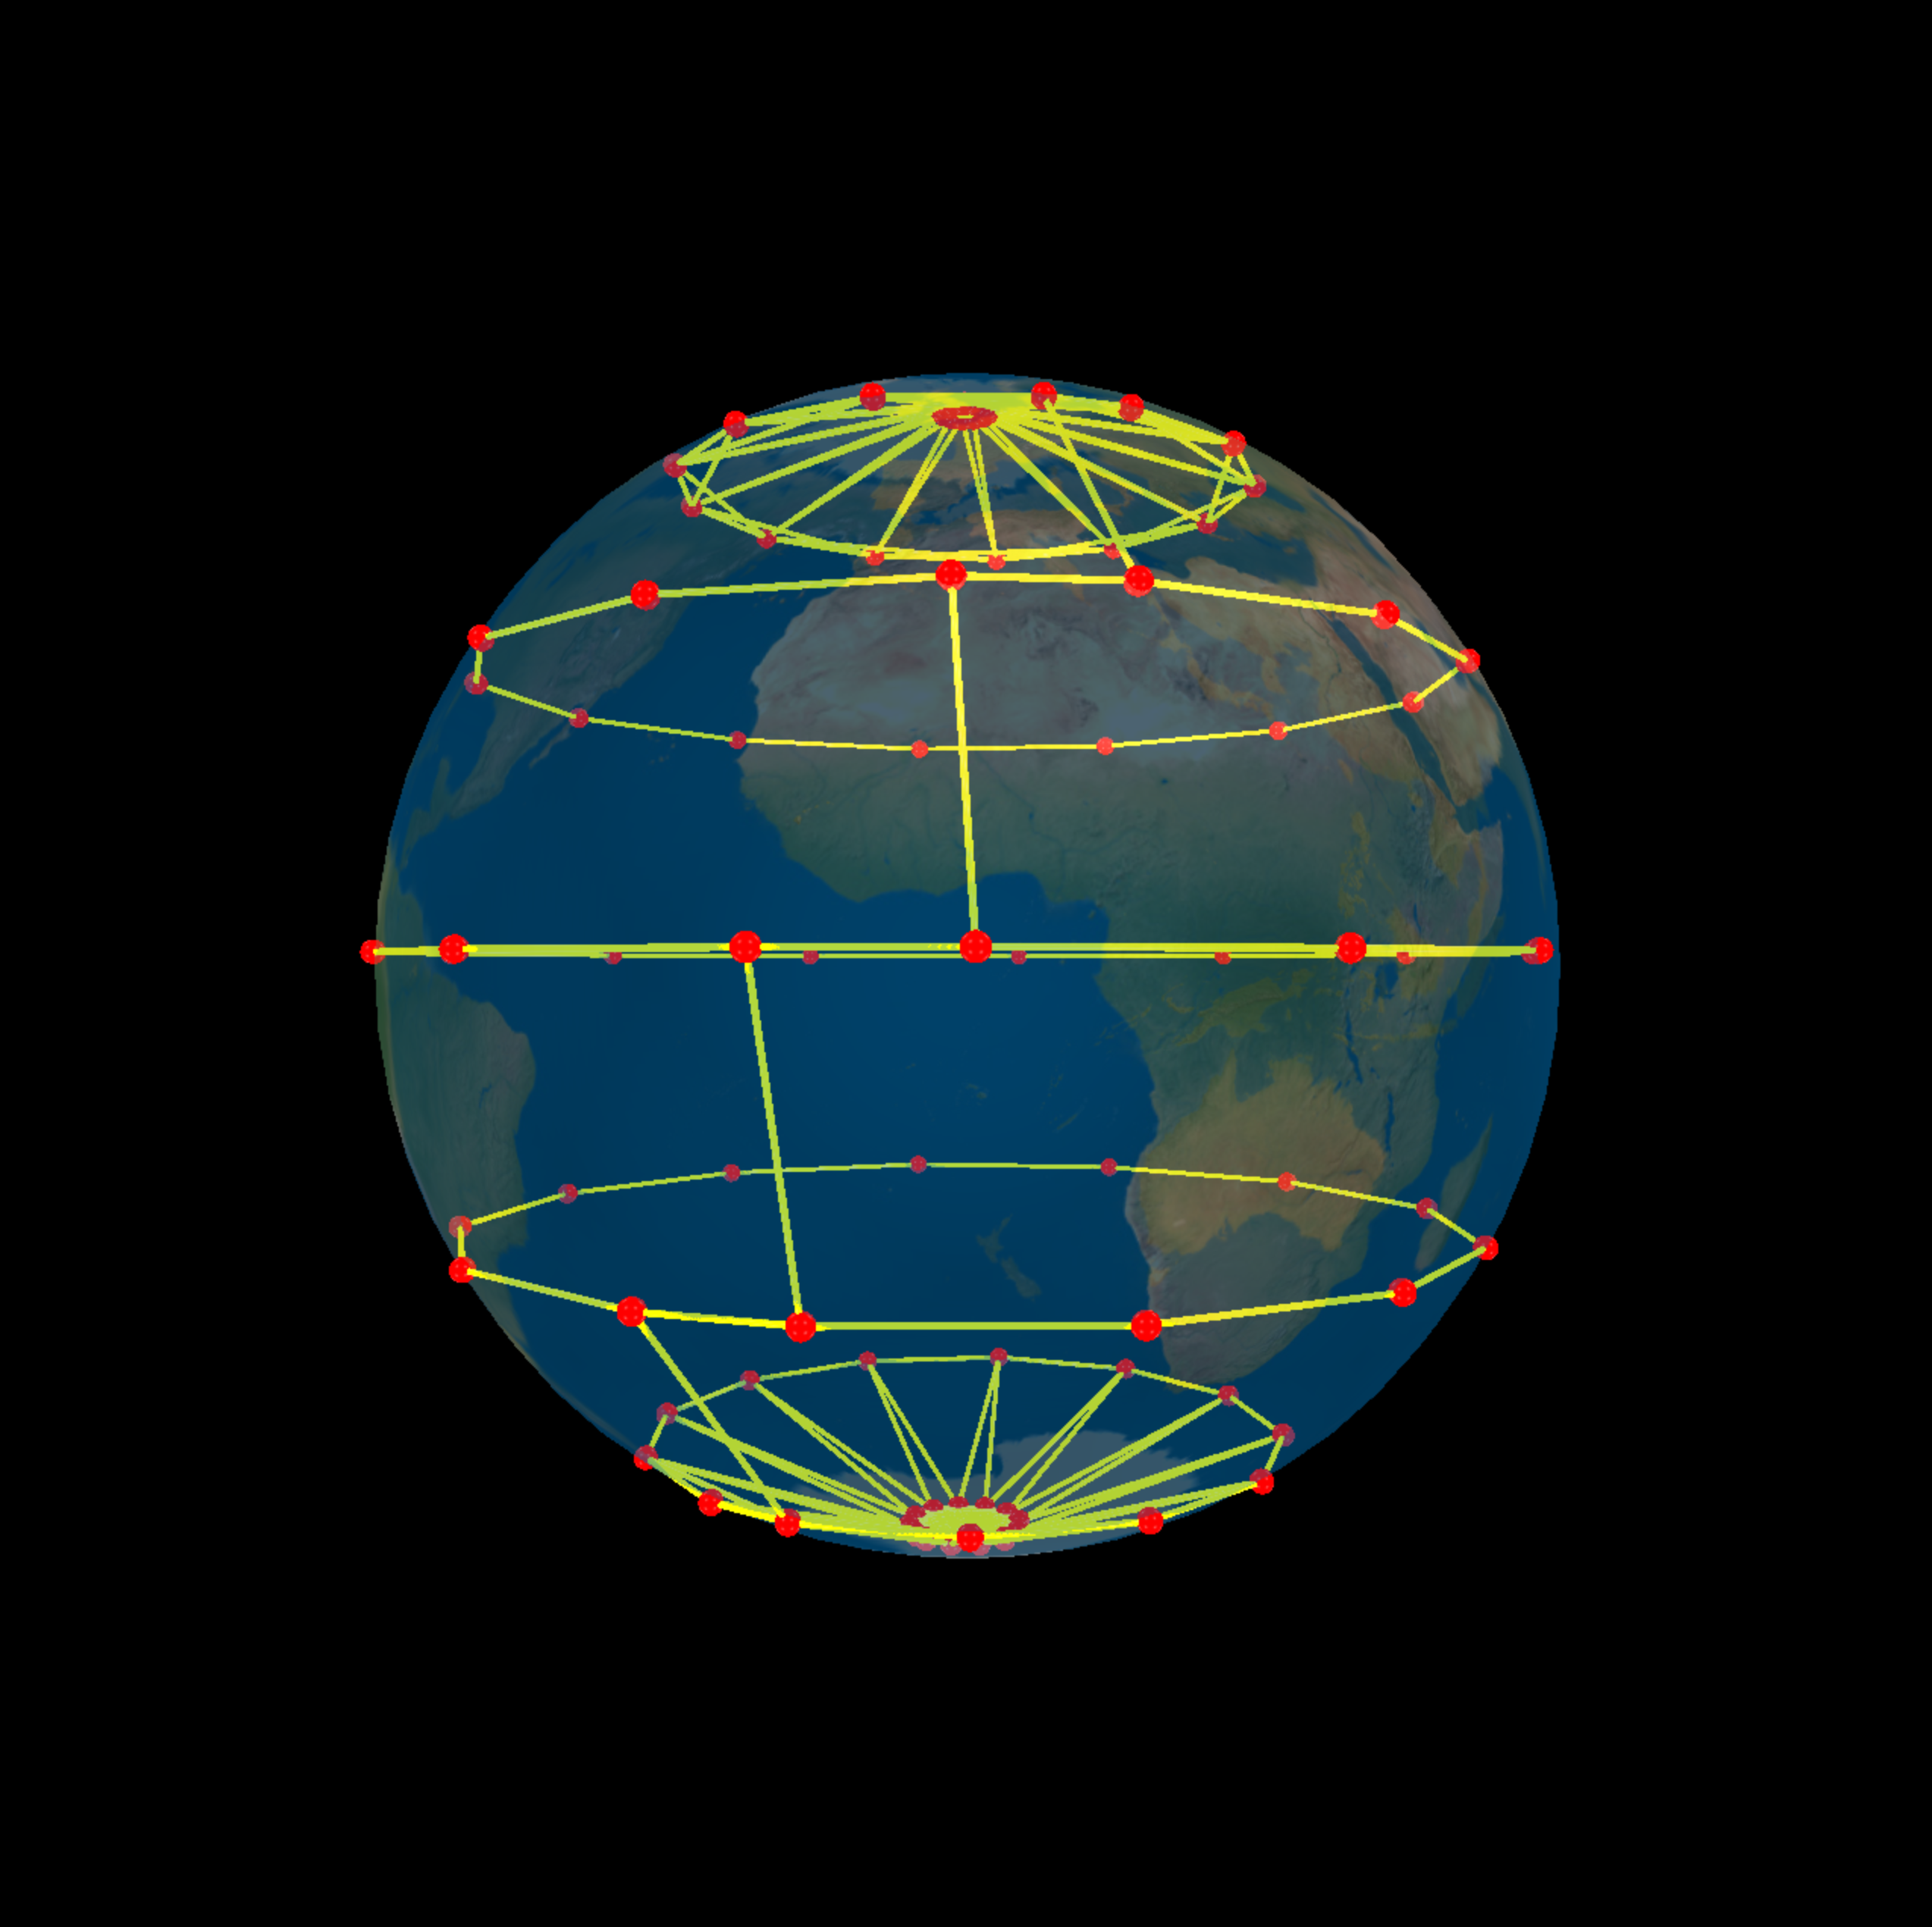
\includegraphics[width=\textwidth]{../images/connections02}
                \caption{sensors02.txt ($r=0.5$)}
            \end{subfigure}
        }
        \caption{Connections between sensors}
\end{figure}

\section{Coverage}
TODO: Cech complex, increasing $r$ until Betti number $b_1$ is 0 (zero cycles/holes). plots (homology, barcode), 3d image

\begin{figure}[H]
        \centering
        \makebox[\linewidth][c]{
        	\centering
            \begin{subfigure}[b]{0.6\textwidth}
                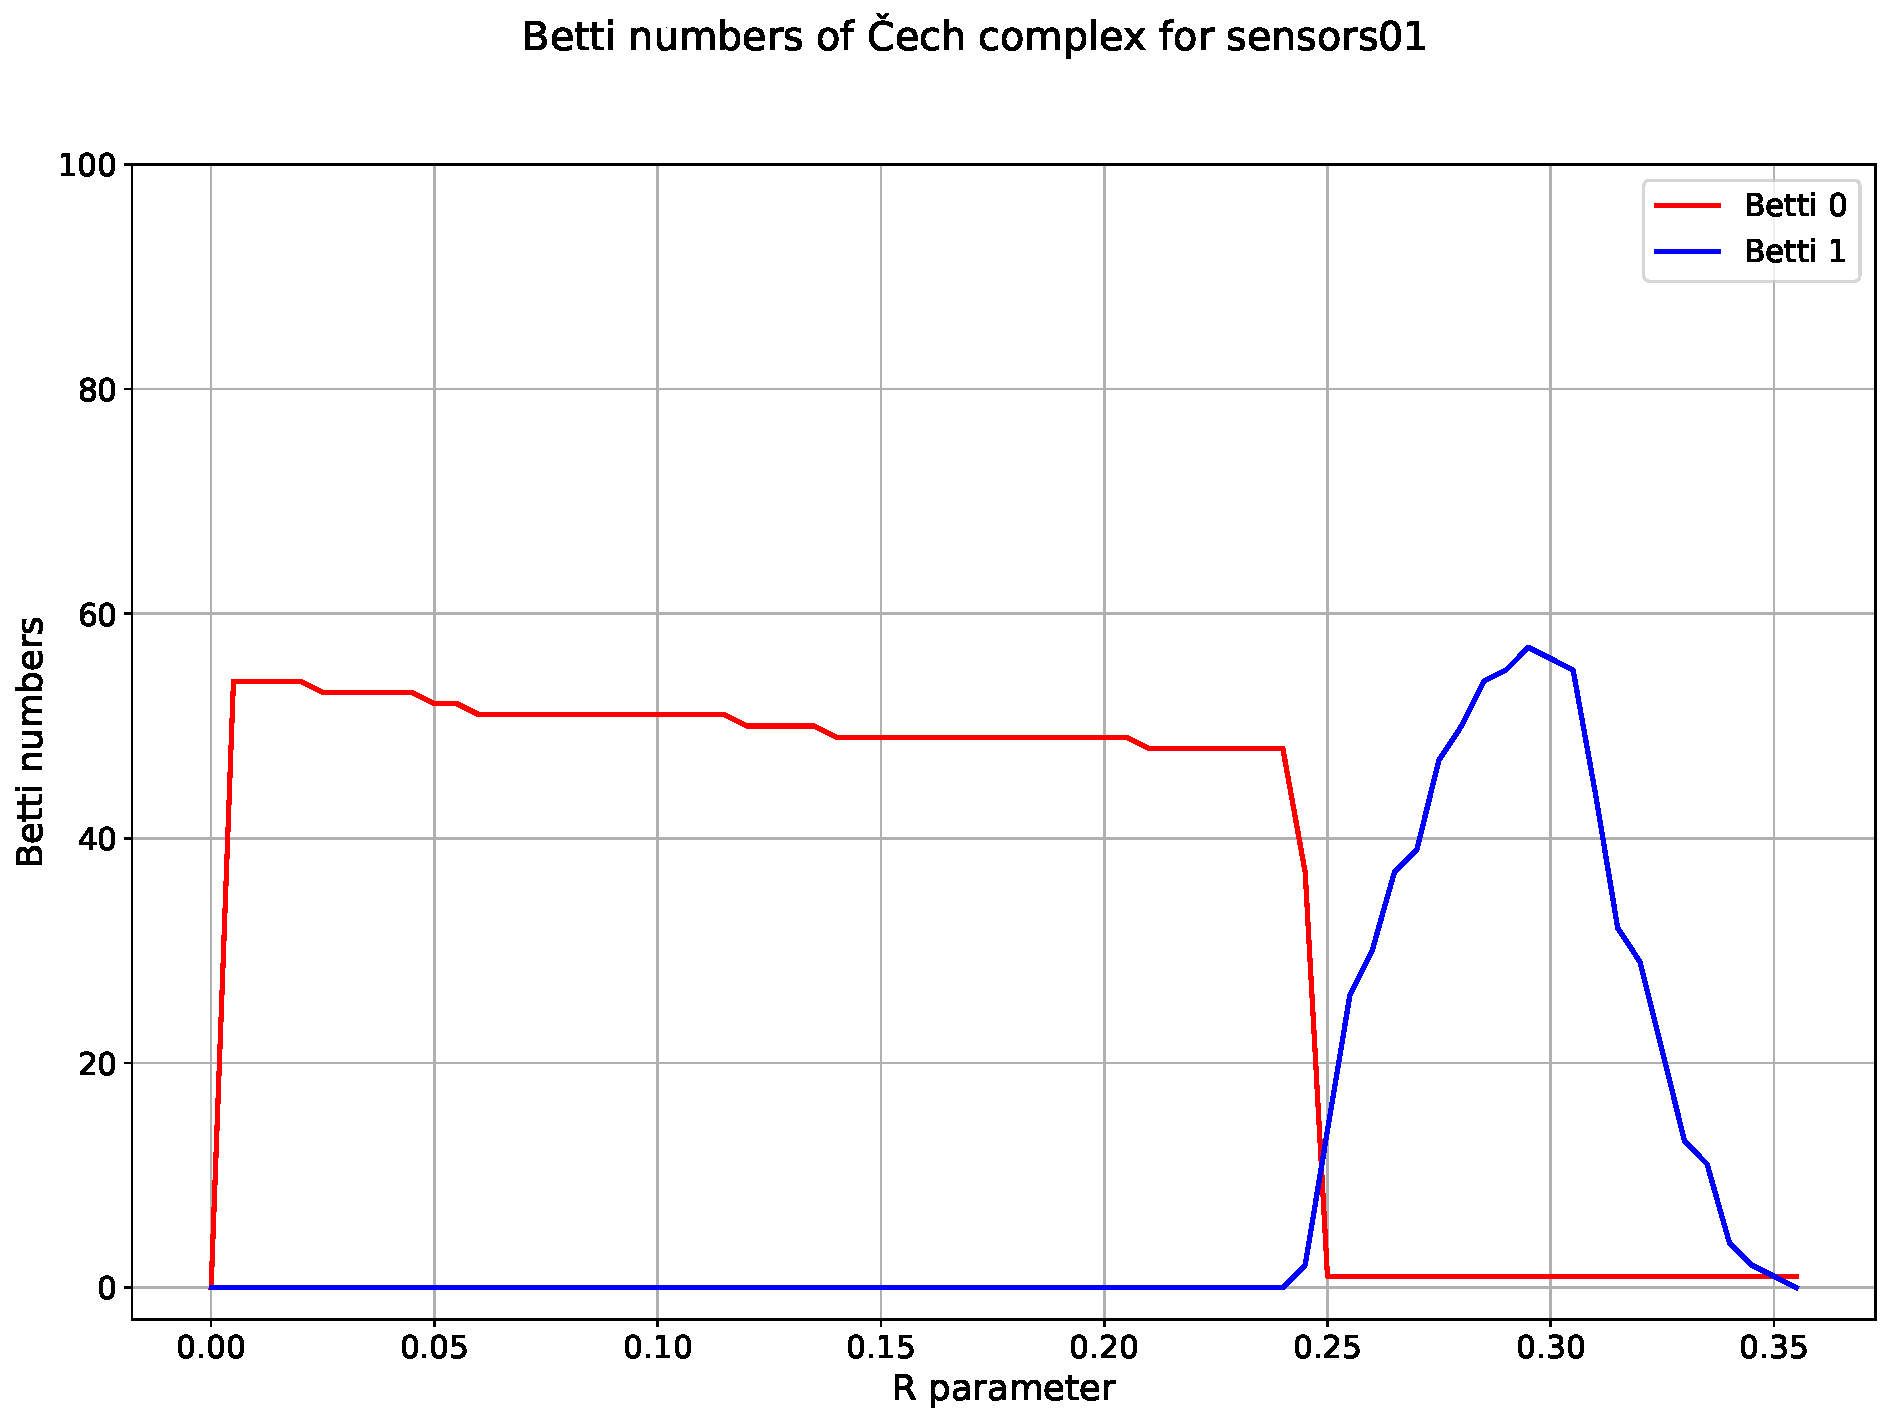
\includegraphics[width=\textwidth]{../images/plot_cech_sensors01}
            \end{subfigure}
            \begin{subfigure}[b]{0.6\textwidth}
                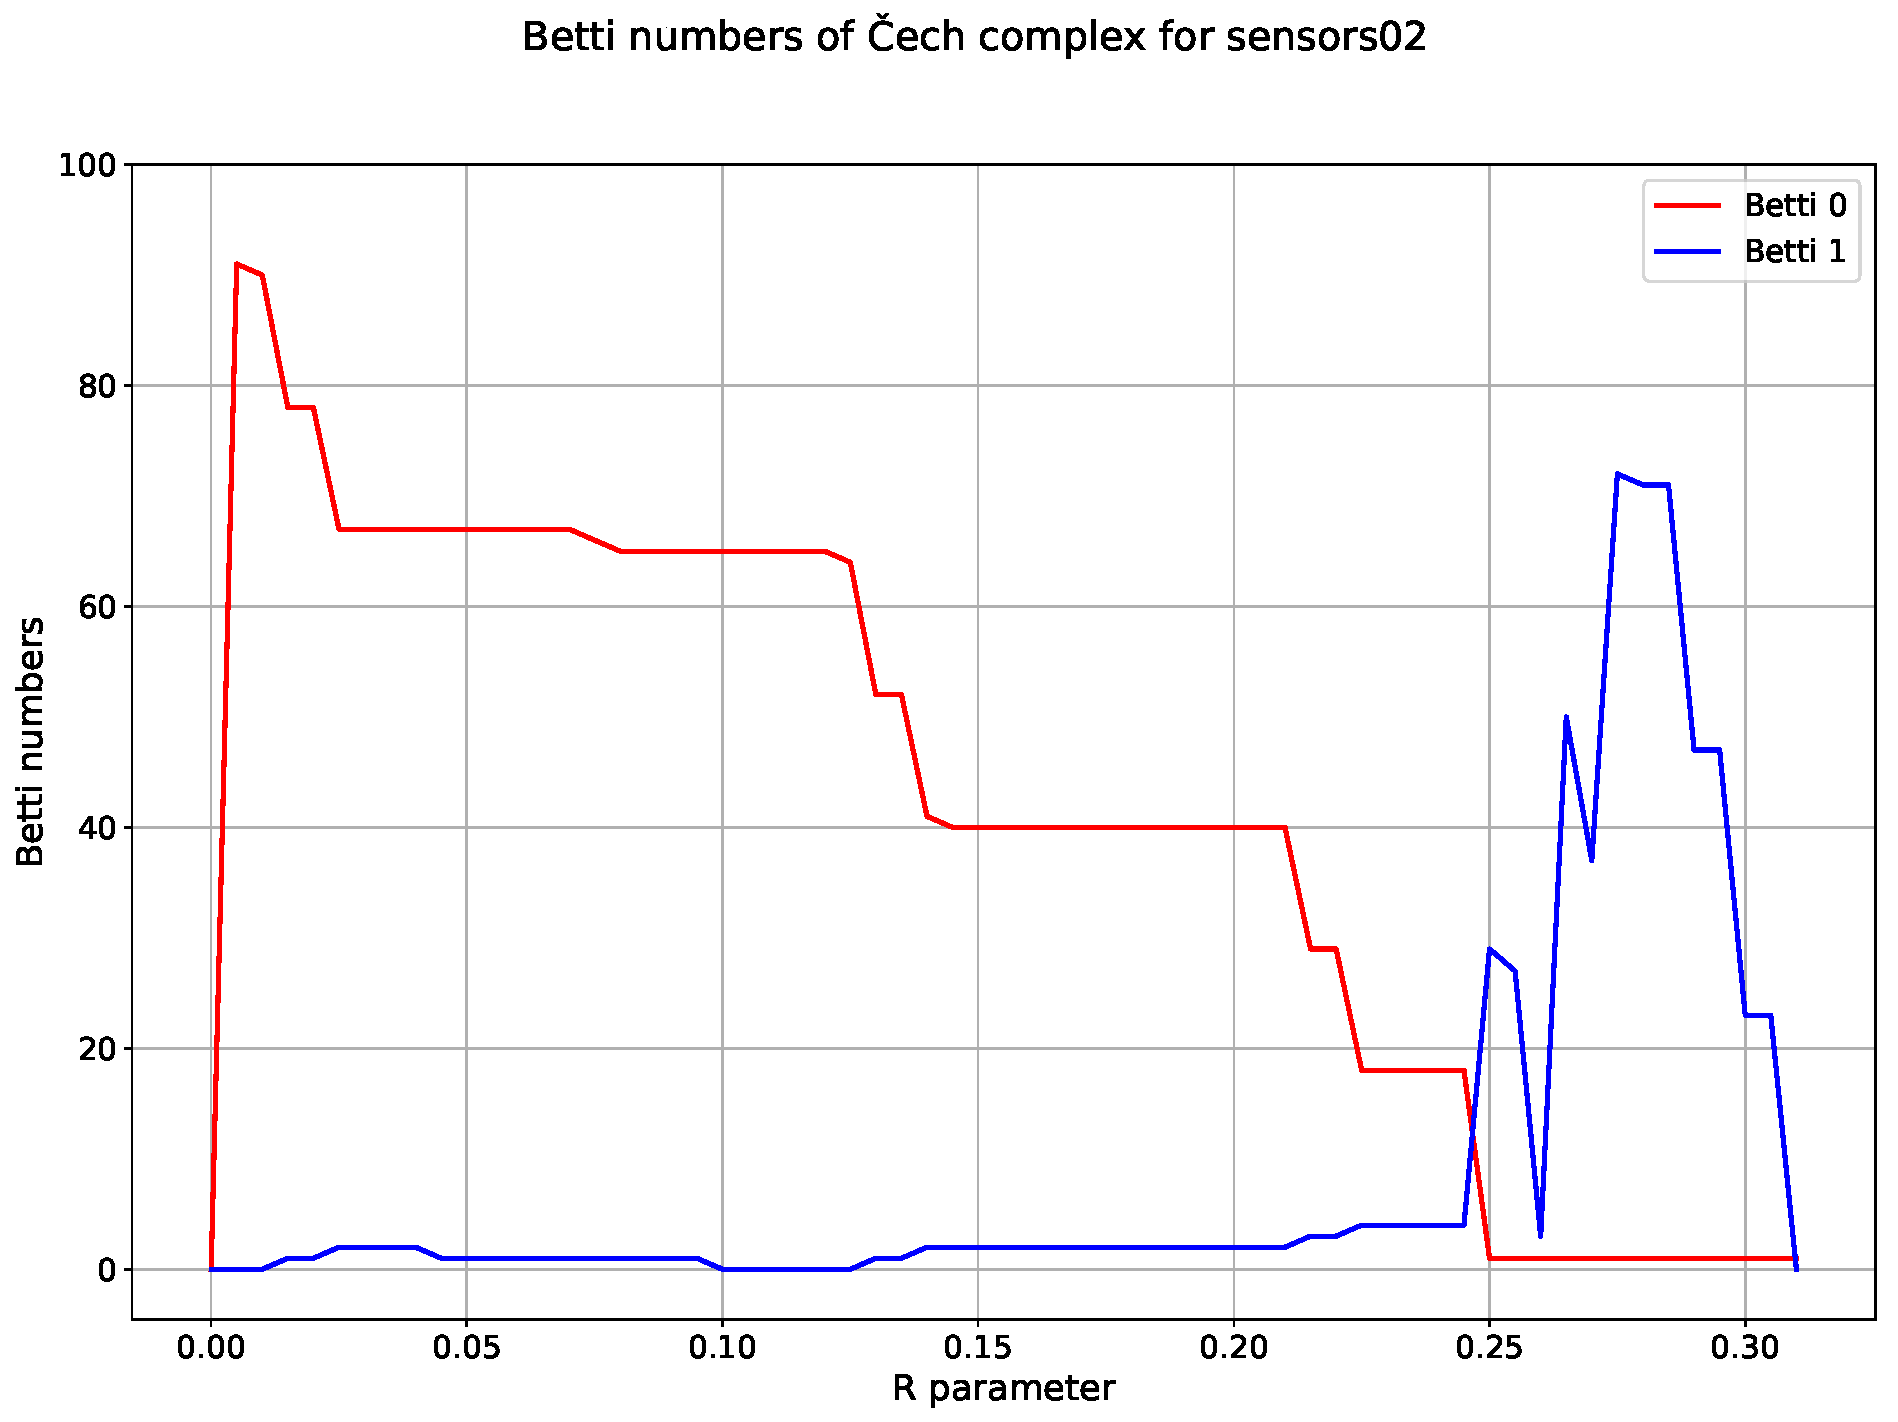
\includegraphics[width=\textwidth]{../images/plot_cech_sensors02}
            \end{subfigure}
        }
        \caption{$b_0$ and $b_1$ as we increase the $R$ parameter}
\end{figure}

\begin{figure}[H]
        \centering
        \makebox[\linewidth][c]{
            \centering
        	\begin{subfigure}[b]{0.6\textwidth}
            	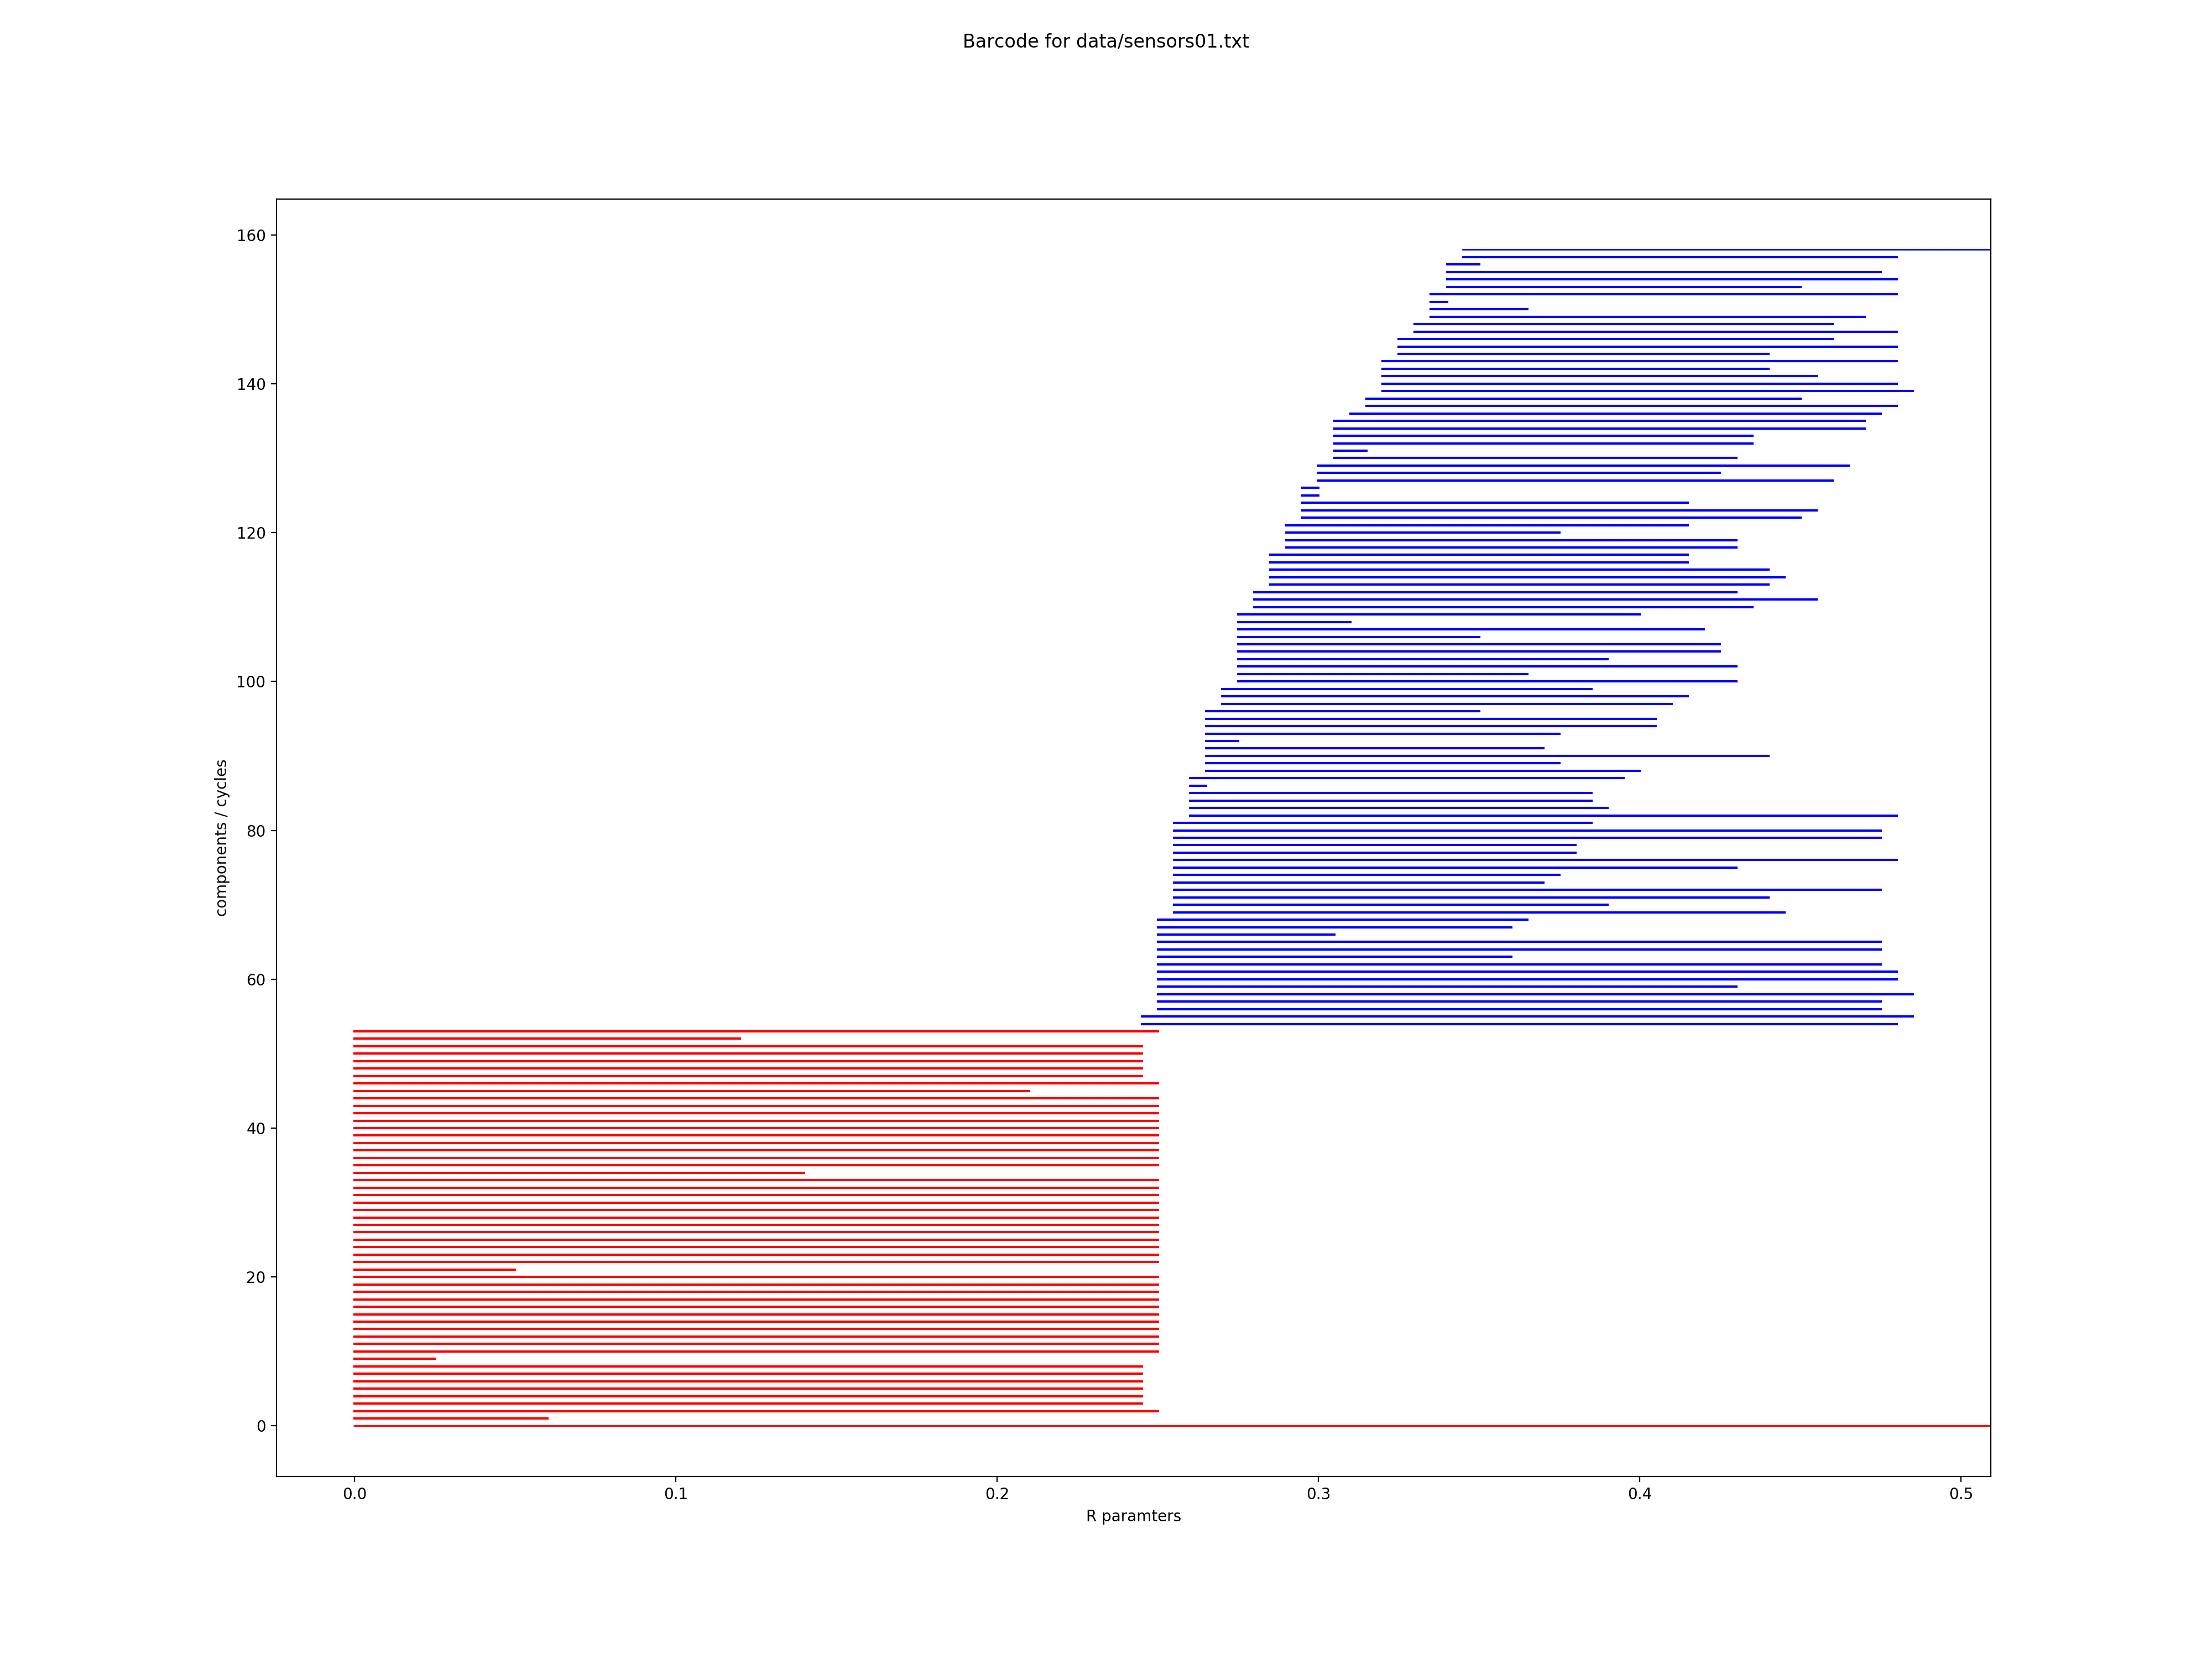
\includegraphics[width=\textwidth]{../images/barcode_cech_sensors01}
        	\end{subfigure}
			\begin{subfigure}[b]{0.6\textwidth}
            	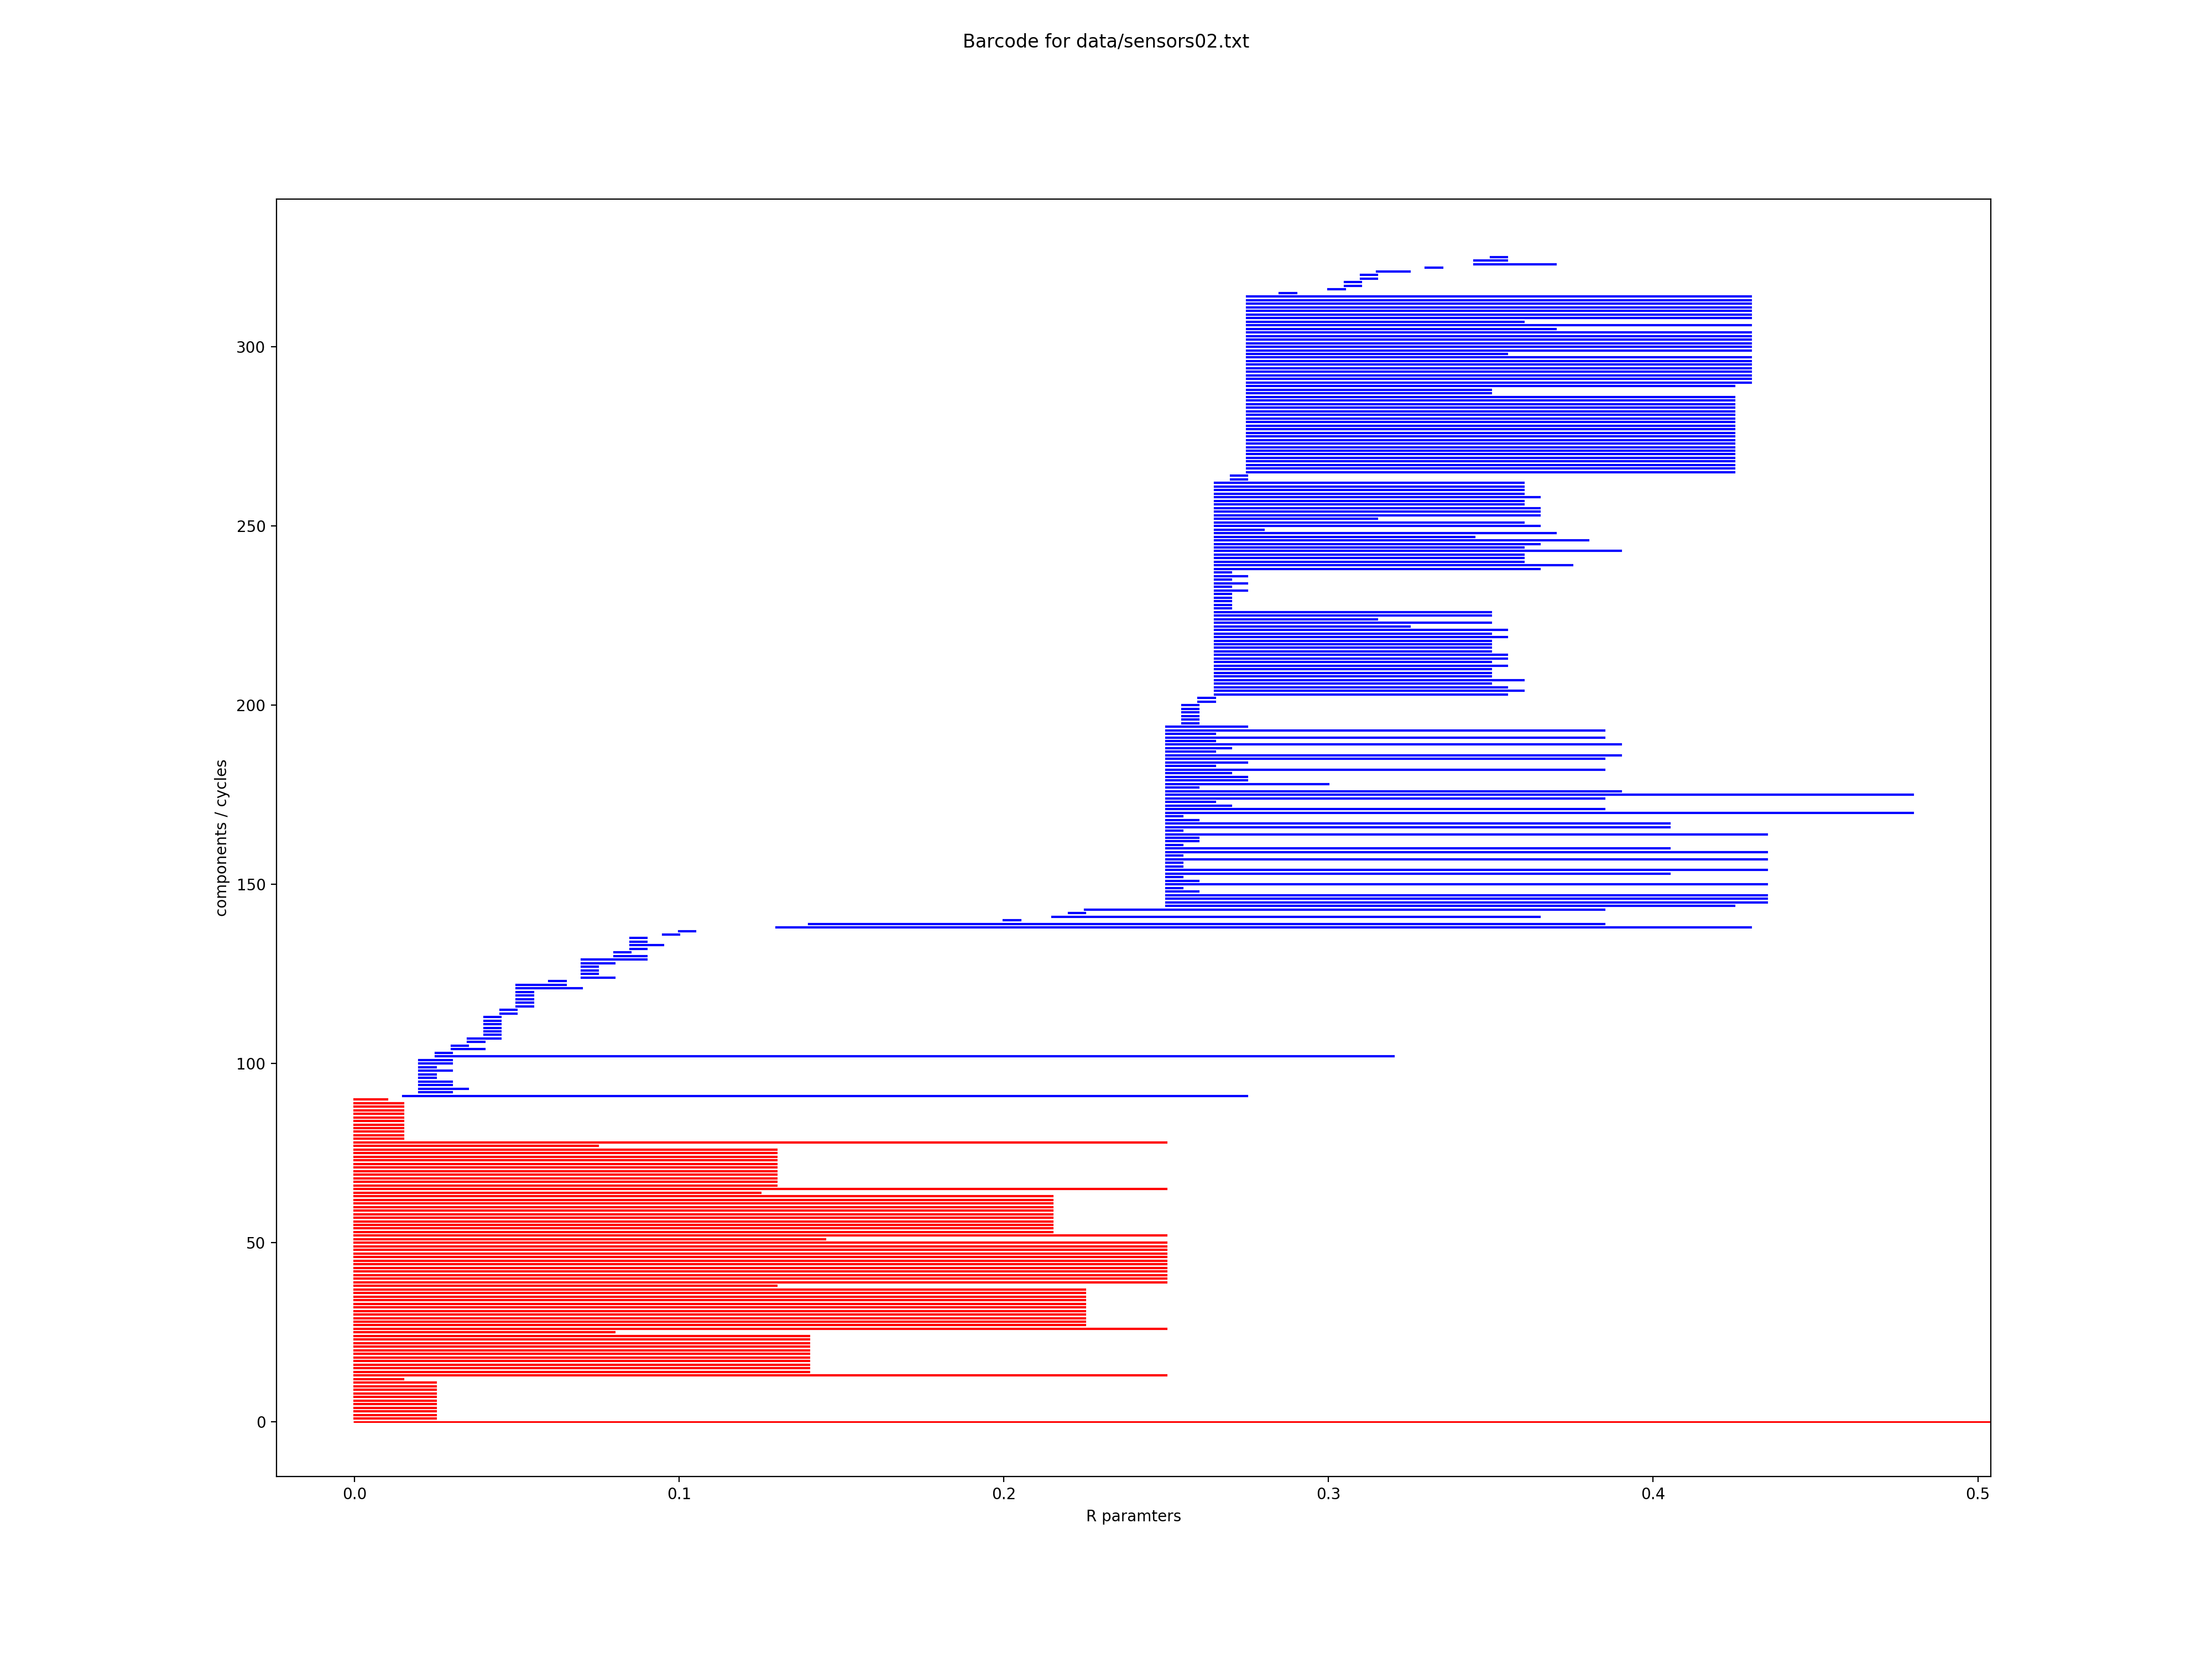
\includegraphics[width=\textwidth]{../images/barcode_cech_sensors02}
        	\end{subfigure}
        }
        \caption{Barcodes for the Čech complex}
\end{figure}

TODO: malo komentarja na graf

\begin{figure}[H]
        \centering
        \makebox[\linewidth][c]{
        	\centering
            \begin{subfigure}[b]{0.55\textwidth}
        	    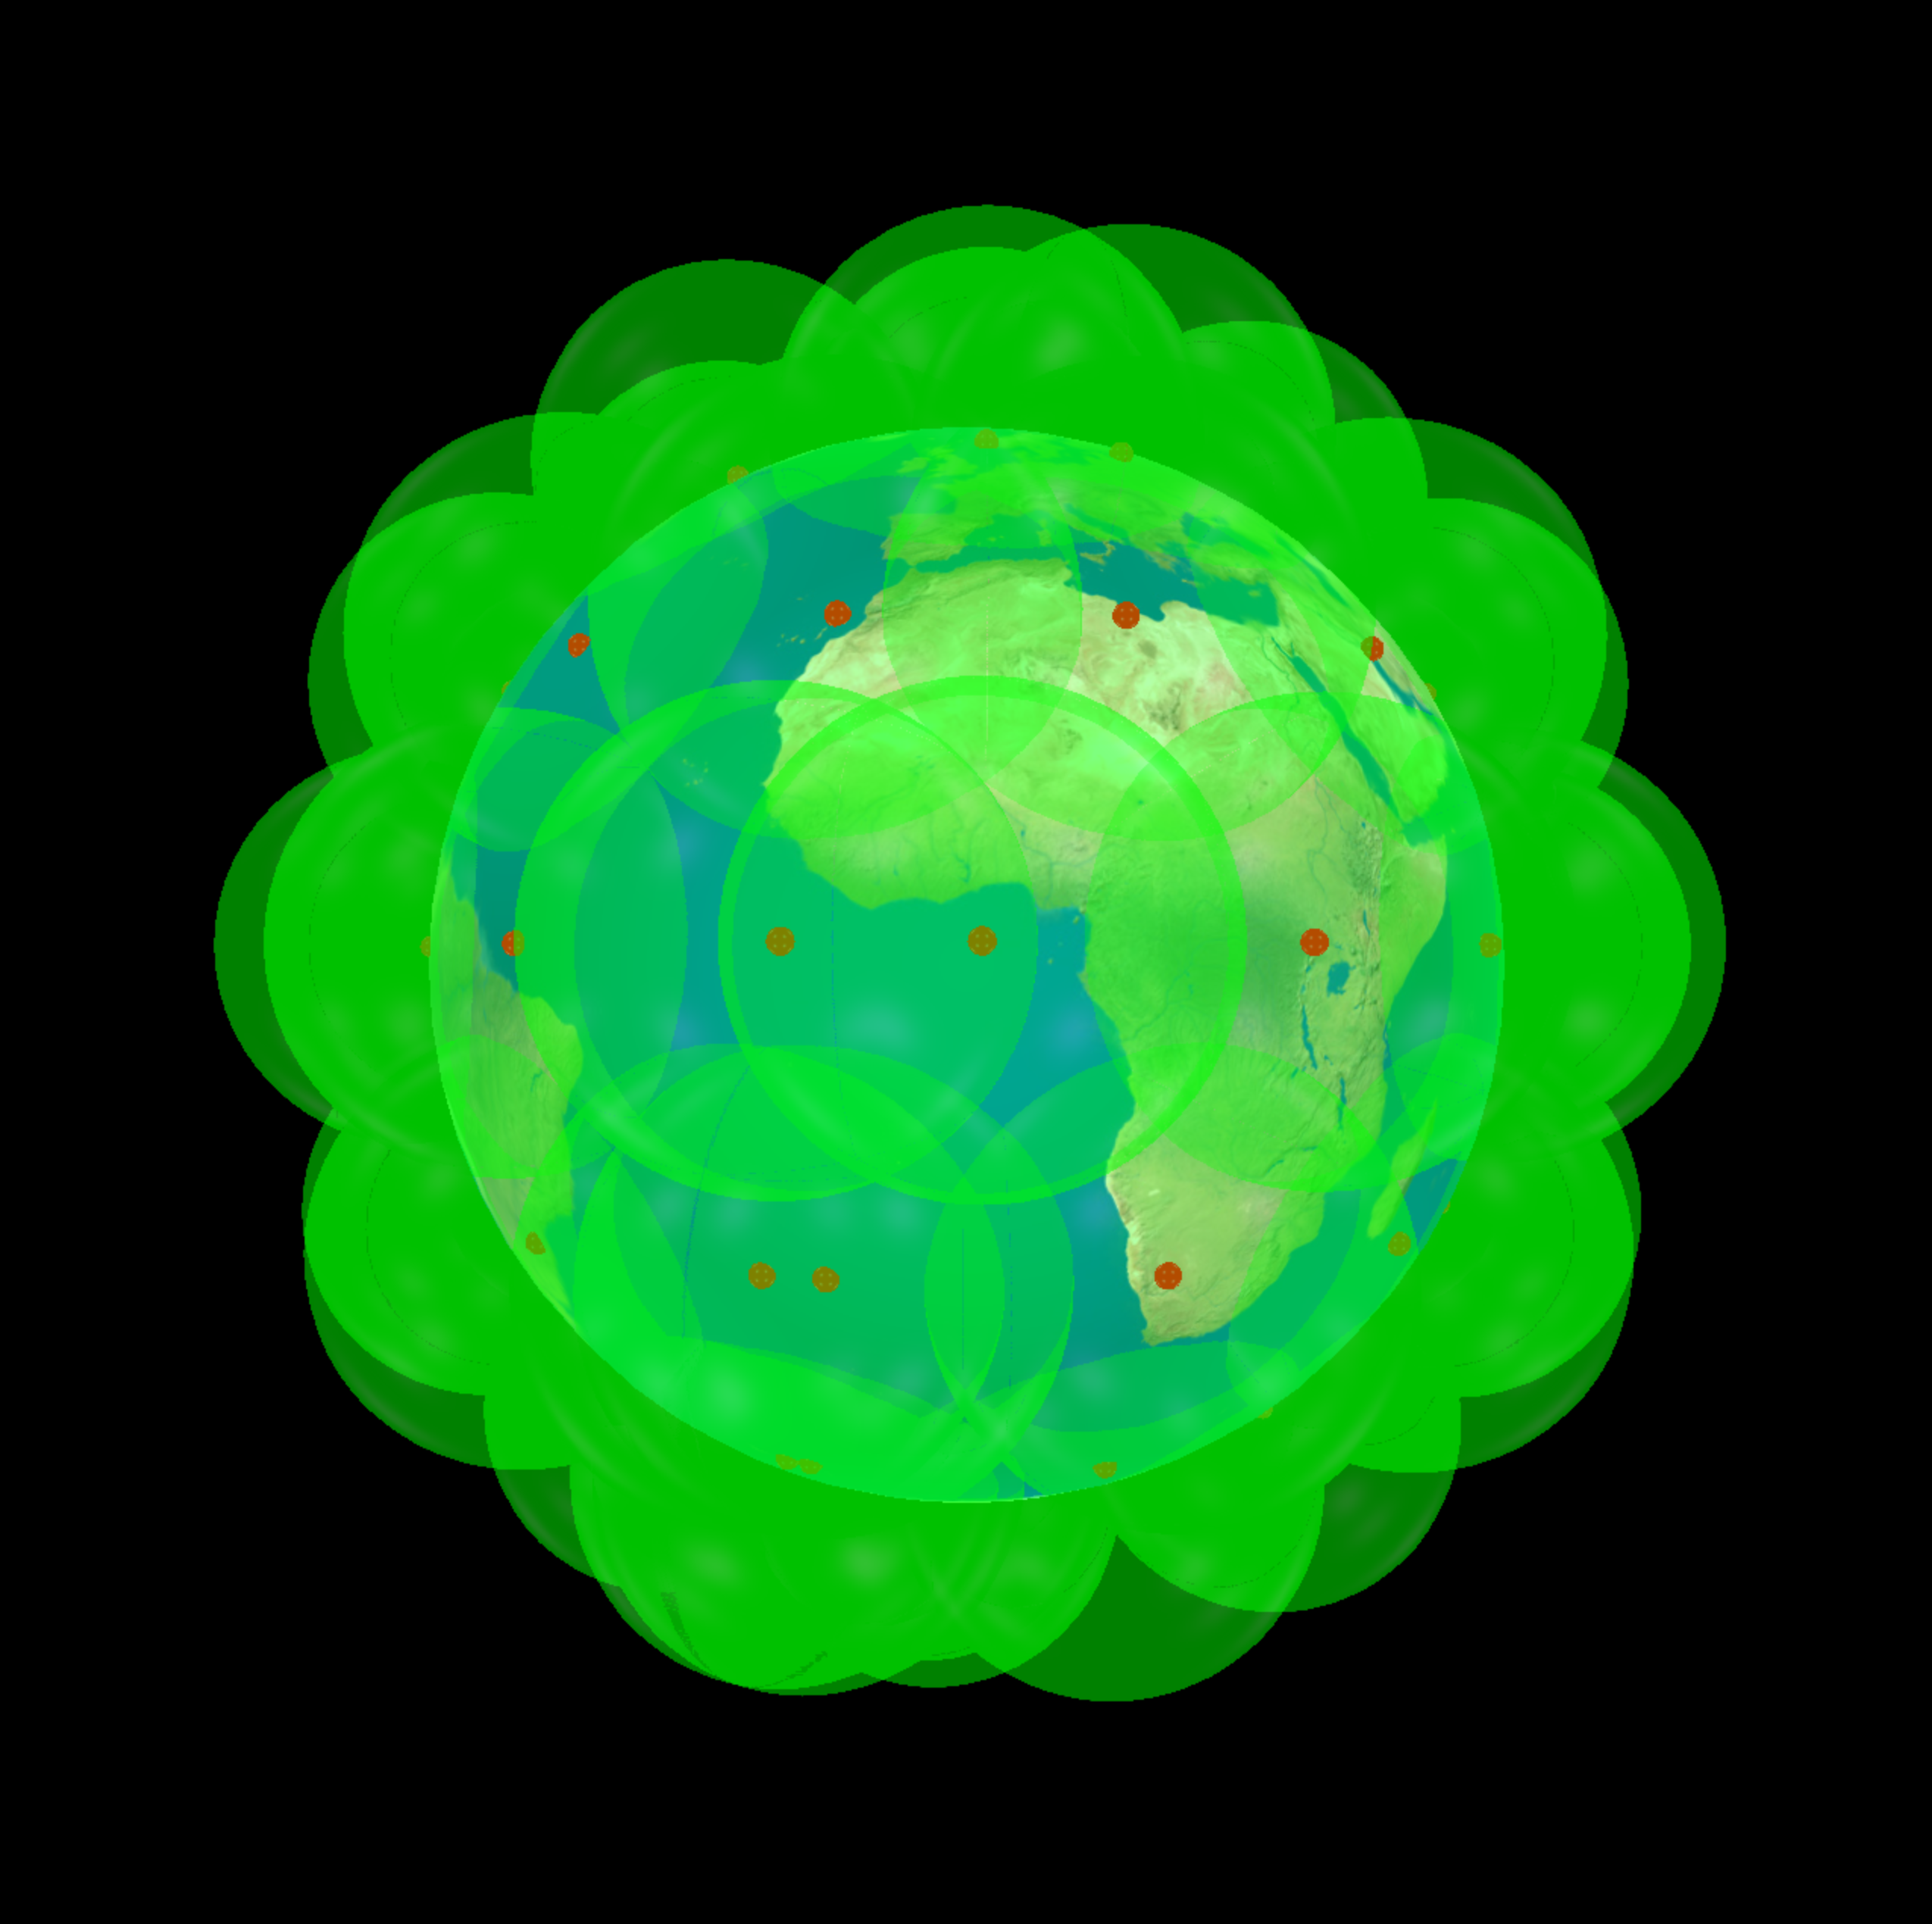
\includegraphics[width=\textwidth]{../images/coverage01}
        	    \caption{sensors01.txt ($R=0.355$)}
        	\end{subfigure}
        	\begin{subfigure}[b]{0.55\textwidth}
      	      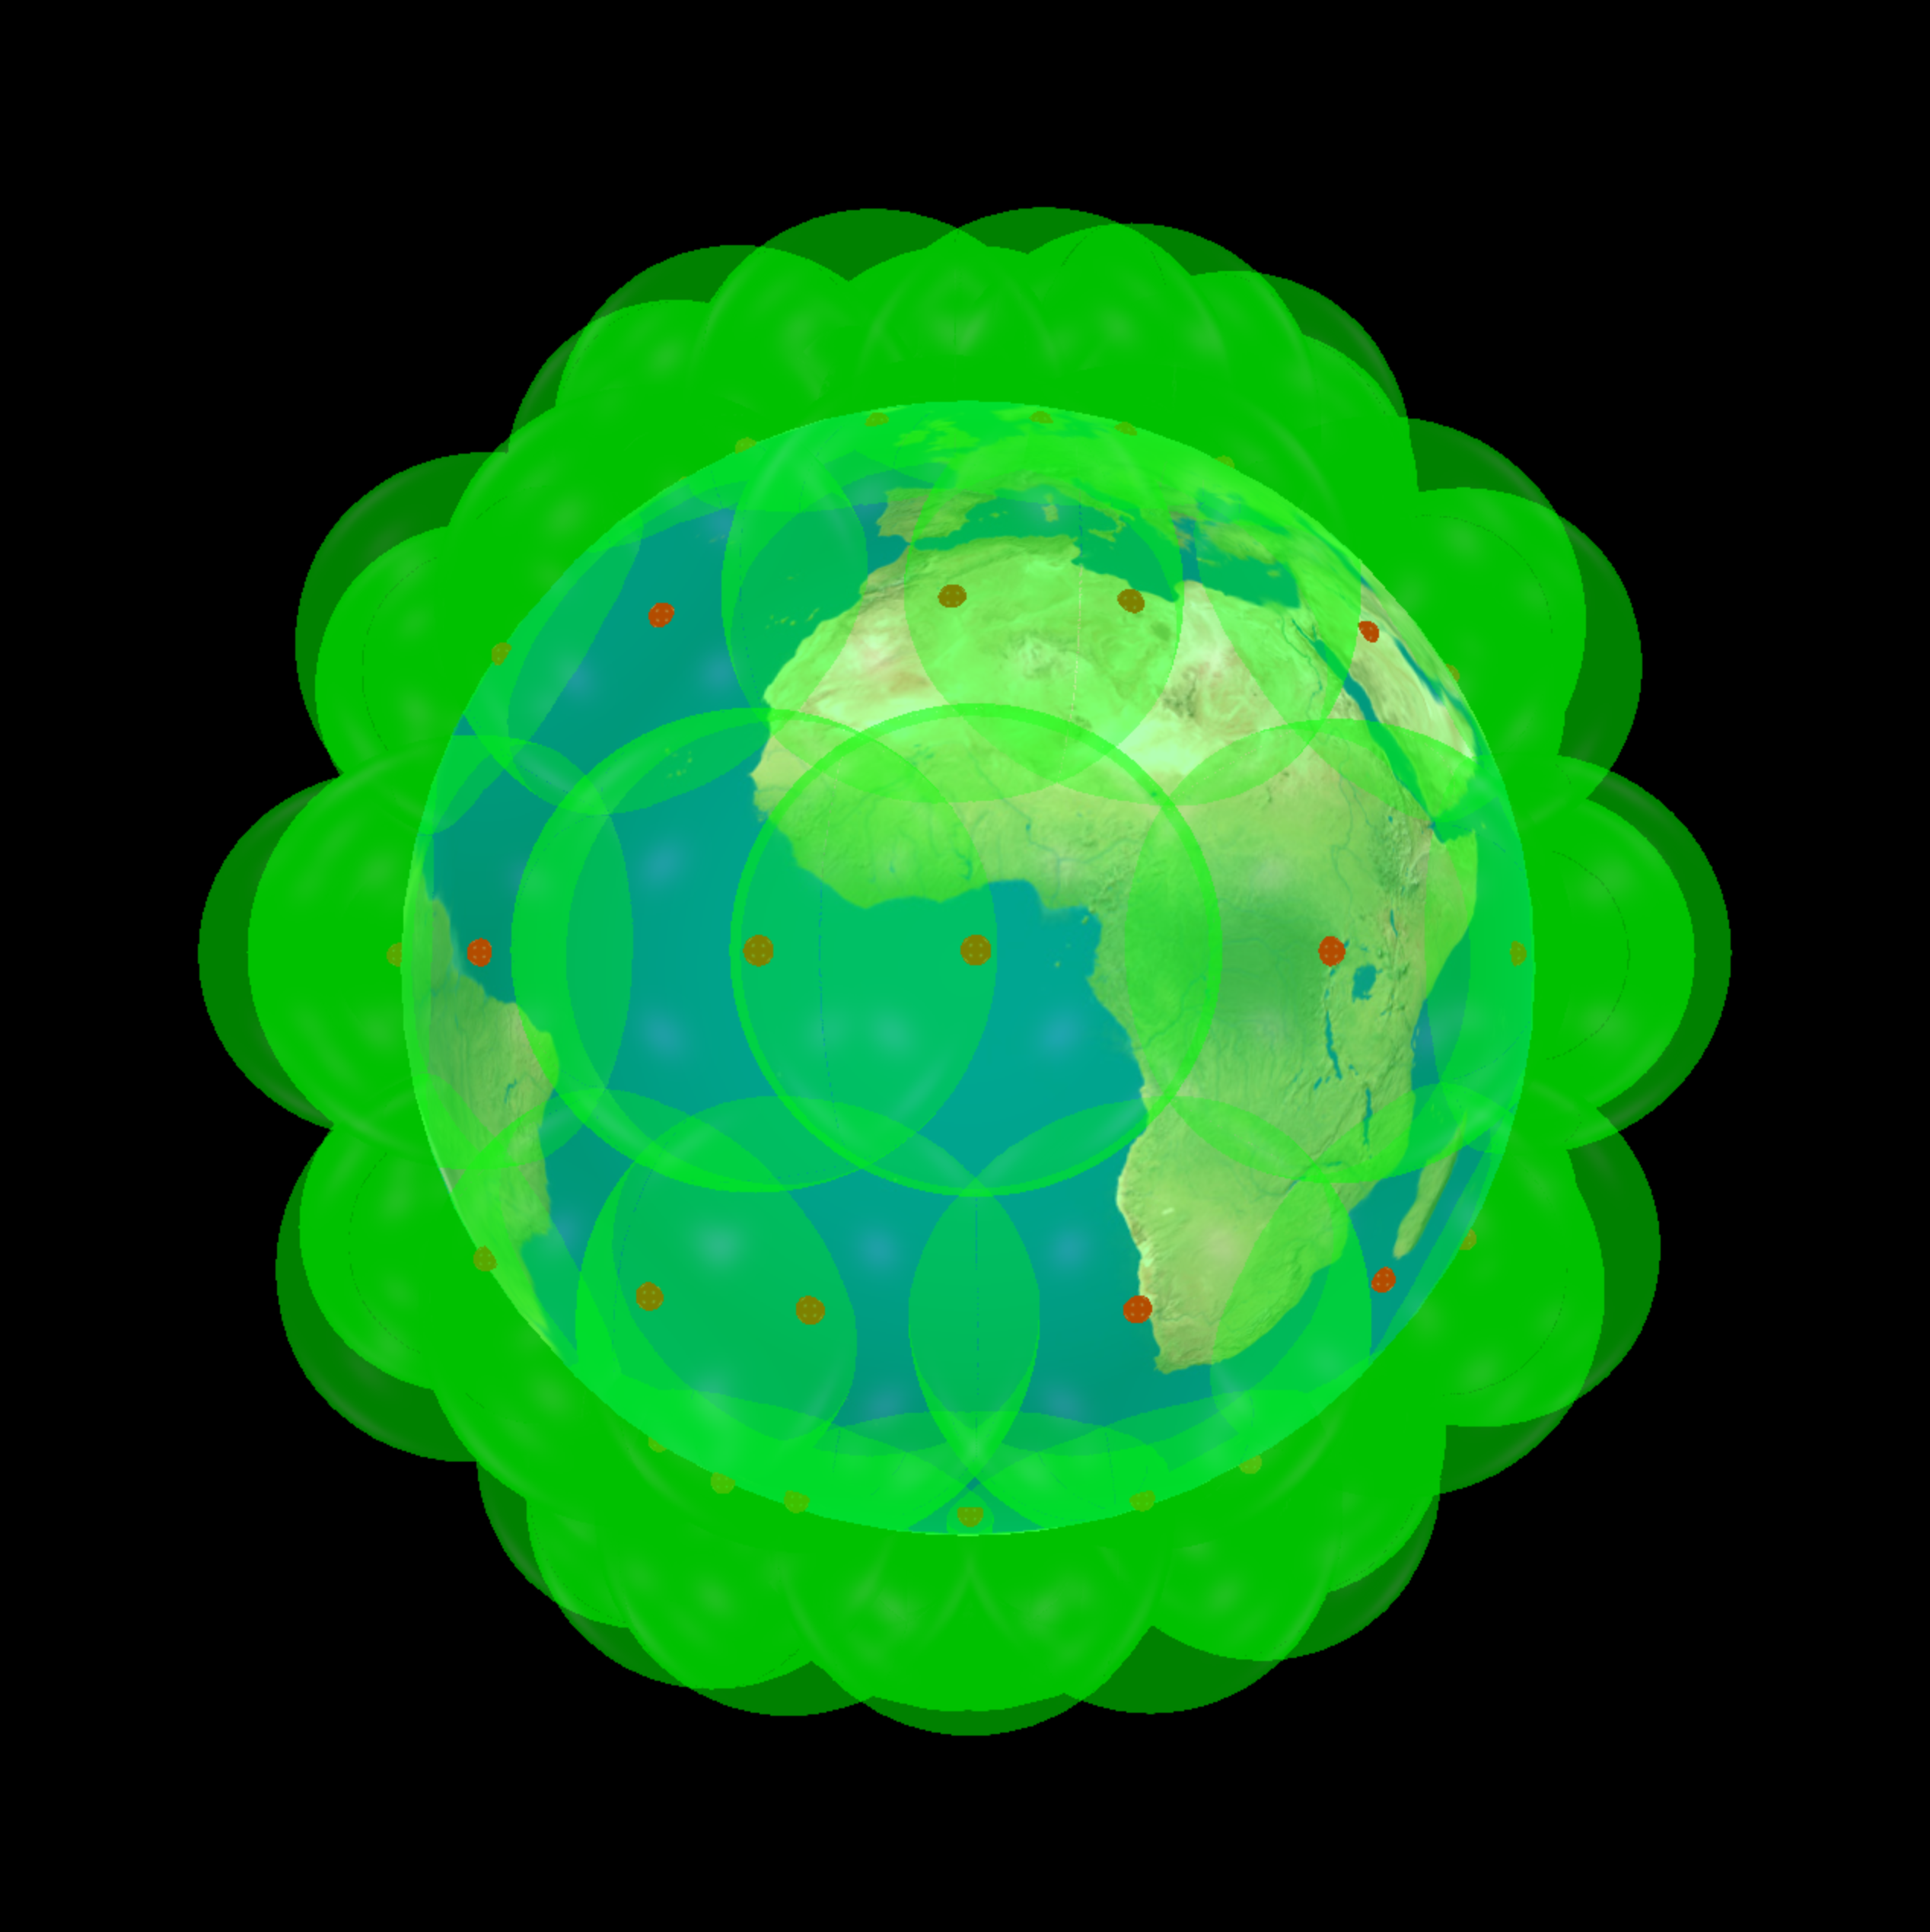
\includegraphics[width=\textwidth]{../images/coverage02}
     	       \caption{sensors02.txt ($R=0.31$)}
     	   \end{subfigure}
	  	}
        \caption{Connections between sensors}
\end{figure}

\section{Data generator}
Lastly, lets have a look at the data generator that distributes $n$ points evenly on the surface of a sphere. In order to meet this requirement we should look on points as electrons that are bound on the surface (i.e in spherical coordinates have fixed radium). The natural state would be the state with the lowest electrostatic-potential energy $V$ (eq. (2)). This is due to the fact that electrons repel from each other according to Coulumbs inverse square law (eq. (1))

\begin{equation}
	|\vect{F_{ij}}| = k_e \frac{e^2}{|\vect{r_i}-\vect{r_j}|^2},
\end{equation}
\begin{equation}
	V = \sum_{i\neq j}V_{ij} \propto \sum_{i\neq j}\frac{1}{|\vect{r_i} - \vect{r_j}|},
\end{equation}
where $k_e$ is Coulumbs constant, $e$ charge of electron and $\vect{r_i}$ local vector for $i-th$ point. It should be emphasized that potential energy was determined as sum of inversed Euclidean distances between all points. 

\subsection{Simulated annealing}
In order to determine the minimum of electrostatic-potential energy (eq. (2)) we used algorithm for simulated annealing with some Monte-Carlo modifications. At the beginning we randomly distributed $n$ points on the surface of a sphere with radium $r$ and selected the initial temperature of the system $T$. In each iteration a random point was chosen (one point was fixed, so $n-1$ available) and moved it according to Gaussian distribution with appropriate parameters ($\mu = 0$ and small enough $\sigma$). After that, the difference in energy was calculated $\Delta E$. If the energy of newly distributed points was less than before (i.e. $\Delta E < 0$) the move was accepted. Otherwise ($\Delta E \geq 0$) the move was accepted with the probability $\exp(\frac{-\Delta E}{T})$. The higher the difference in energy the lower are chances that we accept the change. Similar for the temperature, the lower the temperature the lower is the probability for accepting a bad move. If for a certain temperature $T$ enough changes $N_T$ were accepted, we decrease the temperature $T$ for $\Delta T$. Continue with another (or same) random point.   

\subsection{Generated datasets}

In this report we will include two generated datasets, for $n = 4$ and for $n = 50$. We can see that in case of four points they distribute themselves in tetrahedral geometry and for $n = 50$ we get nice homogeneous even distribution of points.

\begin{figure}[!ht]
	\centering
	\begin{subfigure}{.5\textwidth}
		\centering
		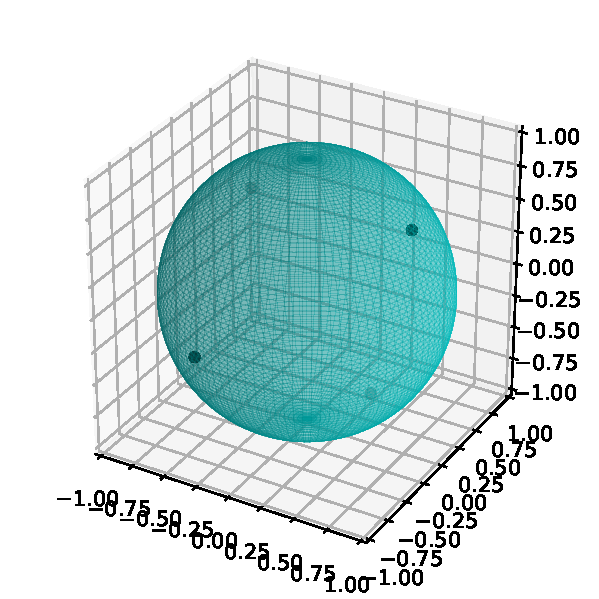
\includegraphics[scale=0.75]{../images/generated2.pdf}
		\caption{n = 4}
	\end{subfigure}%
	\begin{subfigure}{.5\textwidth}
		\centering
		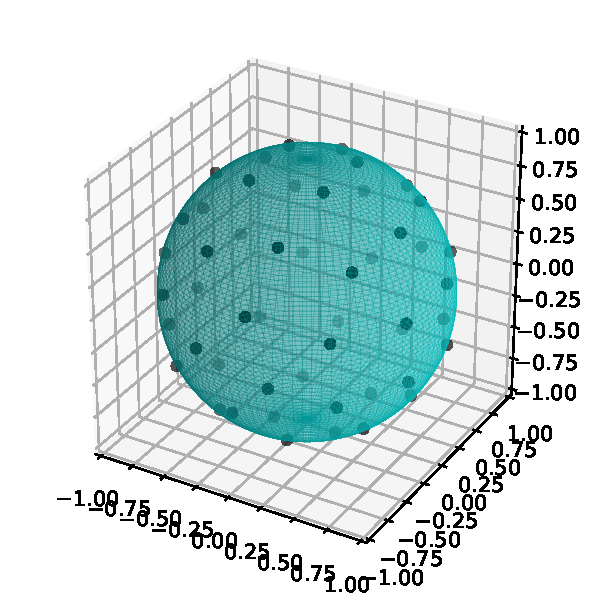
\includegraphics[scale=0.75]{../images/generated1.pdf}
		\caption{n = 50}
	\end{subfigure}%
    \caption{Even distribution of generated $n$ points on the surface of a sphere.}
	
\end{figure}
\section{Redundant sensors}
TODO: how we remove the sensors which are not needed

\section{Conclusion}
TODO

\section{References}
\begin{thebibliography}{99}
	\bibitem{} Vietoris-Rips. \url{https://en.wikipedia.org/wiki/Vietoris_Rips_complex} (5.6.2018).
	\bibitem{A}Čech-complex. \url{https://en.wikipedia.org/wiki/Cech_complex} (5.6.2018).
	\bibitem{A}Dionysus. \url{http://www.mrzv.org/software/dionysus/} (5.6.2018).
	\bibitem{A}Miniball algorithm. \url{https://github.com/weddige/miniball} (5.6.2018).
	\bibitem{A}Vpython. \url{http://vpython.org/} (5.6.2018).
	\bibitem{B} Lecture notes from prof. dr. Neža Mramor Kosta.
\end{thebibliography}


\end{document}
